\documentclass{article}

\usepackage[utf8]{inputenc}
\usepackage[T1]{fontenc} 
\usepackage[italian]{babel}

% --- Matematica e Fisica  ---
\usepackage{amsmath}
\usepackage{amsthm} 
\usepackage{physics}
\usepackage{amssymb}
\let\div\relax
\usepackage{mathabx}

\usepackage{mathtools, cancel, bm}
\usepackage[output-decimal-marker={,}]{siunitx}

% --- Formattazione Testo e Layout ---
\usepackage{ragged2e}
\usepackage{quoting}
\usepackage{sectsty}
\usepackage{booktabs}
\usepackage{enumitem}
\usepackage{array}
\usepackage{tabularx}
\usepackage[a4paper, left=1.5cm, right=1.5cm, top=2cm, bottom=2cm]{geometry} 

% ---  Grafica, Colori e TikZ  ---
\usepackage{graphicx}
\usepackage{float} 
\usepackage{xcolor}
\usepackage{circuitikz}
\usepackage{pgfplots}
\pgfplotsset{compat=1.16} 
\usepackage{tikz}
\usepackage{tikz-3dplot}
\usetikzlibrary{arrows.meta, angles, quotes, trees}
\usepackage[most]{tcolorbox}

\definecolor{RoyalBlue}{RGB}{0, 83, 155}
\definecolor{ForestGreen}{RGB}{34, 139, 34}
\definecolor{CodeBack}{RGB}{245, 245, 245}

% --- Configurazione LISTINGS ---
\usepackage{listings}
\lstdefinestyle{notebook}{
    backgroundcolor=\color{CodeBack},   
    commentstyle=\color{ForestGreen}\itshape,
    keywordstyle=\color{RoyalBlue}\bfseries,
    numberstyle=\tiny\color{gray},
    stringstyle=\color{red!70!black},
    basicstyle=\ttfamily\small,
    breakatwhitespace=false, breaklines=true, captionpos=b, keepspaces=true,                 
    numbers=left, numbersep=5pt, showspaces=false, showstringspaces=false,
    frame=l, framesep=5pt, rulecolor=\color{RoyalBlue},
    language=Python, morekeywords={as, np, plt}
}
\lstset{style=notebook}


\usepackage[colorlinks=true, linkcolor=black]{hyperref} 

\newtcolorbox{nota}{
  blanker,
  before skip=1em,
  after skip=1em,
  left=1em,
  borderline west={1pt}{0pt}{black},
  fontupper=\itshape,
  before upper={\noindent\textbf{Nota}:\quad}
}


\newtcolorbox{definizione}{
  blanker,
  before skip=1em,
  after skip=1em,
  left=1em,
  borderline west={2pt}{0pt}{blue},
  fontupper=\normalfont,
  before upper={\noindent\textbf{Definizione}:\quad}
}


\newtheorem{example}{Example}
\newtheorem{theorem}{Teorema}


\theoremstyle{remark}
\newtheorem{osservazione}{\textbf{\color{ForestGreen}Osservazione}}

% --- Configurazione Intestazioni  ---
\usepackage{fancyhdr}
\pagestyle{fancy}
\fancyhf{}
\fancyhead[L]{\small \nouppercase{\leftmark}}
\fancyhead[R]{\small \thelezione}
\fancyfoot[C]{\thepage}

\newcommand{\thelezione}{}

% --- Comando Lezione 2025  ---
\newcommand{\lezione}[2]{
\newpage
\renewcommand{\thelezione}{#2} 
\section{#1} 
\noindent\textbf{\color{RoyalBlue}Lezione del #2}\par\vspace{0.5em}\hrule\vspace{1em}
}


% --- Comando Ripasso Bressan (Rosso - Subsubsection inline) ---
\newcommand{\ripasso}[1]{
    % Crea una subsubsection colorata in rosso
    \subsubsection{\texorpdfstring{\color{red}Parte di Bressan: #1}{Parte di Bressan: #1}}
}

\title{\textbf{\Huge Appunti di Statistica}}
\author{\textsc{Mirolo Manuele / Alessio Brusini / Michele Tedeschini}}
\date{a.a. 2025/26}

% --------------------------------------------------

\begin{document}
\maketitle
\justifying

\newpage 
\begin{center}
\section*{Premessa}
Le sotto sezioni in Rosso sono quelle che riguardano il ripasso di Bressan, tutte le altre (in nero) sono quelle che riguardano il programma dell'anno attuale.    
\end{center}

\tableofcontents
\newpage

\textit{Se noi non fossimo ignoranti non ci sarebbe probabilità, ci potrebbero essere solo certezze. Ma la
nostra ignoranza non può essere assoluta, altrimenti non ci sarebbe più probabilità. Così i problemi di
probabilità possono essere classificati a seconda della maggiore o minore profondità della nostra
ignoranza.\\
(H. Poincaré)}

\setcounter{section}{-1}
\section{Contatti e informazioni}
\begin{itemize}
    \item Mail: agata.trovato@units.it
    \item Ufficio: Edificio F, primo piano, Aula 114
    \item Ricevimento: Giovedì dalle 14:00 alle 1:00
\end{itemize}

\lezione{Introduzione / Ripasso di Bressan}{2024}

La probabilità è la misura del grado della credenza che un certo evento avvenga.

L'oggetto della teoria è un certo \textit{esperimento causale}, la cui esecuzione è detta \textit{prova}, il risultato è indicato con \textit{$\omega$}, l'insieme di
tutti gli $\omega$ possibili è detto \textit{spazio campione $\Omega$}. Un \textit{Evento A} è un sottoinsieme di $\Omega$, se $\omega$ $\in$ A allora esso realizza l'Evento.
Se esso è l'unico elemento costituente di A allora esso è l'\textit{evento elementare}, altrimenti A è un \textit{evento composto}.
Altre nomenclature sono legate alla teoria insiemistica (per esempio due eventi A e B sono disgiunti se l'insieme A non interseca l'insieme B).
\subsection{Definizioni di probabilità}
Si possono dare due definizioni di probabilità:
\begin{description}

\item[CLASSICA]: dato uno spazio \textbf{finito} $\Omega$, la probabilità è il rapporto:

\[
P(E)= \frac{\text{casi favorevoli}}{\text{casi possibili}}
\]

Questa funzione è utile quando i casi risultano essere \textbf{ugumente possibili}.

\vspace{0.5cm}

\item[FREQUENTISTICA]: emerge dal ragioanamento fondato sui risultati di un esperimento:
\[
P(E)=\lim_{N \rightarrow \infty} \frac{n}{N}
\]

dove $n$ è il numero di volte che si verifica un evento, mentre N è le volte che viene ripetuto l'esperimento.
\end{description}


\subsection{Definizione assiomatica di probabilità}
Dato un evento A $\subseteq \Omega$ la misura di probabilità $P$ è una funzione $P:\Omega \rightarrow \mathbf{R}  $ le cui caratteristiche sono:



\begin{itemize}
    \item $P(A) \geq 0$
    \item $P (evento \hspace{0.1cm} certo)=1$
    \item  Se A e B sono eventi \textbf{disgiunti} (incompatibili), cioè $P(A \cap B) = 0$, allora $P(A \cup B) = P(A)+P(B)$, che nella forma generalizzata risulta essere:
    \[
    P(\bigcup_{i=1}^{\infty}A_i)=\sum_{i=1}^{\infty}P(A_i)
    \]
\end{itemize}

\subsection{Proprietà della misura di probabilità}
\begin{itemize}

    \item Probabilità negazione: $P(\overline{A})=1-P(A)$
    \item Estremi della misura di probabilità: $0 \leq P(A)\leq 1$
    \item Teorema delle probabilità totali (con $A \bigcap B \neq 0$): 
    \[
    P(A \cup B)=P(A)+P(B)-P(A \cap B)
    \]
    \[
    P(A - B)=P(B)-P(A \cap B)
    \]
    \item Probabilità in relazione d'inclusione (con $A\subseteq B$): $P(A)\leq P(B)$
\end{itemize}


\subsubsection{Probabilità condizionata}

La probabilità che si verifichi $A$ se si verifica $B$: 
\[
P(A|B)=\frac{P(A \bigcap B)}{P(B)}
\]

Il \textbf{Teorema delle probabilità totale} mi enuncia che se ho che se ho n eventi e si ha che 
\[ \displaystyle P(M_i \cap M_j)=0 \hspace{0.3cm}\forall i \neq j \hspace{0.5cm} \& \hspace{0.5cm} \bigcup_{i=0}^{n}M_i=\Omega \]
dove $\Omega$ è lo spazio campione; allora:
\[
P(A)=\sum_{i=1}^{n}P(A|M_i)P(M_i)
\]
Mentre per l'indipendenza si ha $P(A \cap B)=P(A)P(B)$

\subsubsection{Probabilità delle cause}
Ci chiediamo quale sia la probabilità che $M_j$ sia la causa di un certo evento $A$.


\subsection{Teorema di Bayes }
Dato un certo set di ipotesi ($M_i$) e un certo evento $A$ il teorema mi dice come la probabilità a "posteriori" $P(M_i|A)$ cambia dopo che l'evento $A$ si è verificato.

Consideriamo un eveneto $A$ e una classe completa di ipotesi ($M_j$):
\[
\begin{cases}
    M_i\bigcap M_j=0 \\
    \bigcup_j M_j=\Omega
\end{cases}
\]
 
Utilizzando il teorema della probabilità condizionata e il fatto che $P(A \bigcap M_i)=P(M_i \bigcap A)$ posso ricavare la probabilità che una causa sia dovuta a un determinato evento
\[
P(M_i|A)=\frac{P(A|M_I)P(M_i)}{P(A)}=\frac{P(A|M_i)P(M_i)}{\sum_{j=1}^{n}P(A|M_j)P(M_j)}
\]
Dove:
\begin{description}
    \item[P(M)]: probabilità a priori/margianale (non tiene conto di A)
    \item [P(M \textbar \space A)]: probabilità condizionata/a posteriori, nota A
    \item [P(A \textbar \space M)]: probabità condizionata di A, nota M
    \item [P(A)]: è la probabilità di A a priori, serve da costante di normalizzazione
\end{description}




\subsection{Indipendenza}
Si dicono due eventi indipendenti: $P(A \cap B)=P(A) \cdot P(B)$ e quindi $P(A|B)=P(A)$ 

Per esempio: nella misura del pendolo fermare il pendolo ad ogni misura rende le misure indipendenti fra di loro (una misura di un periodo sbagliato non influisce sulla misura successiva).

\subsection{Cenni di calcolo combinatorio e fattoriale}
Si chiama combinazione semplice quella in cui non importa l'ordine degli elementi e il numero di combinazioni $C_{n,r}$ è dato da:

\[
C_{n,r} = \binom{n}{r} = \frac{n!}{r!(n - r)!}
\]

Con la definizione di fattoriale:

\[
n! = \prod_{k=1}^{n} k = 1 \cdot 2 \cdot 3 \cdots n = \prod_{i=0}^{n-1} (n - i)
\]

Fattoriale di un numero negativo:
\[
n!=\prod_{i=0}^{n-1}(n-i)
\]
\[
{(c)}^n n!=\prod_{i=0}^{n-1}c(n-i)
\]
\[
{(-1)}^n n!=\prod_{i=0}^{n-1}-1(n-i)=(-n)!
\]

Fattoriale di un numero positivo:
\[
x! = \Pi(x)=\int_{0}^{\infty}t^{x}e^{-t}dt
\]
Che presenta la proprietà:
\[
\Pi(x+1)=(x+1)\Pi(x)
\]

Sempre Eulero introdusse la funzione Gamma $\Gamma$, con uno spostamneto di unità nelle variabili rispetto a $\Pi$:
\[
\Gamma(z)=\int_{0}^{\infty}t^{z-1}e^{-t}dt
\]
Difatti questa funzione è legata a $\Pi$ da $\Pi(x)=\Gamma(x+1)=x\!$ e vale che $z\Gamma(z)=\Gamma(z+1)$

Da questa funzione sono definte le combinazioni semplici del tipo:
\[
\binom{z}{k}=\frac{\Gamma(z+1)}{k\! \Gamma(z-k+1)}
\]

Importanti relazioni tra le funzioni Gamma sono:
\[
\Gamma(z)\Gamma(1-z)=\frac{\pi}{\sin(\pi z)} \hspace{1.5cm} \Gamma(z)\Gamma(-z)=-\frac{\pi}{\sin(\pi z)}
\]
Da queste ricavo che $\Gamma(\frac{1}{2})=\sqrt{\pi}$ e $\Gamma(-\frac{1}{2})=-\sqrt{\pi}$, l'ultima importante relazione è invece:
\[
\Gamma(n+\frac{1}{2})=\frac{(2n-1)!!}{2^n}\sqrt{\pi}
\]



\subsection{Variabili casuali e funzione di ripartizione}
Dato lo spazio di eventi elementare $\omega$ una \textit{variabile casuale} è una funzione $X$ tale che $X(\omega)=x$ dove $x\in$ R,
dunque una funzione che mi prende un campione casuale dal mio spazio campionario e gli associa un numero(ex: valore, altezza, \ldots).

Essa può essere discreta (numerabile) oppure continua, se almeno idealmente posso considerare $\Omega$ continuo.

\subsubsection{Funzione di ripartizione}
Data una variabile casuale $X$, la funzione $F$ che fa corrispondere a un valore x la probabilità cumulativa $P(X \geq x)$ viene detta funzione di ripartizione

\[
F_X:\mathbf{R} \rightarrow [0,1] \; F_X(x)=P(X \leq x)
\]

La funzione di ripartizione è definita sia per le variabili casuali discrete che per le variabili casuali
continue.

Proprietà delle funzioni di ripartizioni:
\begin{enumerate}
    \item $0 \geq F_X(x) \geq 1$
    \item nel caso che il dominio sia \textbf{R}, allora $\displaystyle \lim_{x \rightarrow -\infty} F_X(x)=0 \; e \; \lim_{x \rightarrow \infty}F_X(x)=1$
    \item È una funzione monotona crescente;
    \item \( P(x_1 < X \leq x_2) = F_X(x_2) - F_X(x_1) \) dunque la funzione di ripartizione consente di stabilire la probabilità che la variabile casuale semplice \( X \) 
    assuma valori compresi in intervalli di tipo \((x_1, x_2]\) dove \( x_1, x_2 \in \mathbf{R} \), con \( x_1 < x_2 \). A partire da questo posso calcolare anche le altre probabilità, ad esempio:  
    \[ P(x_1 \leq X < x_2) = F_X(x_2) - F_X(x_1) + P(X = x_1) - P(X = x_2)\]
 
    \item Nel caso di una variabile casuale discreta, la funzione di ripartizione è continua a destra:  
    \[ \lim_{x \to x_0^+} F_X(x) = F_X(x_0).\]  
    mentre a sinistra abbiamo una discontinuità di 1° specie (o salto):  
    \[ \lim_{x \to x_0^-} F_X(x) \neq F_X(x_0)\]  
    Questo è dovuto al fatto che la probabilità di un evento elementare è diversa da zero, quindi la funzione di ripartizione ha un salto in corrispondenza di ogni valore che può assumere la variabile casuale discreta (pensa lancio dei dati dove cambia la probabilità)
\end{enumerate}

In un intervallo posso avere una \textbf{Probabilità uniforme}, ossia eventi in cui la funzione di probabilità è costante (ex nel caso dei dadi la funz. di ripartizione è a gradini)

\subsection{Densità di probabiità}

 Data la variabile casuale continua \( X: \Omega \to \mathbf{R} \) che associa valori dallo spazio campionario all'intervallo 
 \((a, b)\), con \( -\infty \leq a < b \leq +\infty \), la funzione di densità di probabilità (PDF) o funzione di distribuzione di probabilità è 
 la funzione \( f_X: \mathbf{R} \to \mathbf{R}^+ \) che ad ogni \( x \) associa il limite per \( dx \rightarrow 0\), del rapporto tra la probabilità 
 che la variabile casuale assuma valori nell'intervallo \((x, x + dx]\) e l'ampiezza \( dx \), ovverosia possiamo supporre la probabiità che un certo 
 evento cada in un intervallo.

 In simboli:
 
 \[ f_X: \mathbf{R} \to \mathbf{R}^+ : x \mapsto \lim_{dx \to 0} \left[ \frac{P(x < X \leq x + dx)}{dx} \right] = \lim_{dx \to 0} \frac{F_X(x+dx)- F_X(x)}{dx}\]

 Ogni evento deve essere ricondotto all'unione, negazione o intersezione di intervalli del tipo $( -\infty, x] $

 \textbf{Attenzione} a non confondere la funzione di densità con una probabilità.
 Essa mi determina la densità di probabilità che la variabile casuale sia nell'intervallo $dx$.

 Definimamo la \textbf{Funzione di distribuzione cumulativa}:
 \[
 F(x)=\int_{x_{min}}^x f_X(t)dt
 \]


\begin{center}
\begin{tikzpicture}[scale=1.5]
    
    % Asse x
    \draw[->] (-0.5,0) -- (4,0) node[right]{$x$};
    % Asse y
    \draw[->] (0,-0.5) -- (0,3) node[above]{$y$};
    
    % Etichette
    \node at (1.5,-0.2) {$a$};
    \node at (3,-0.2) {$b$};
    \node at (0.7,2.5) {$y = f_X(x)$};
    
    % Curva della PDF
    \draw[domain=0.5:3.5, smooth, variable=\x, blue] plot ({\x}, {2.5*exp(-0.5*(\x-2)^2)});
    
    % Area evidenziata
    \fill[blue!20] (1.5,0) -- plot[domain=1.5:3, smooth, variable=\x] ({\x}, {2.5*exp(-0.5*(\x-2)^2)}) -- (3,0) -- cycle;
    
    % Linee verticali
    \draw[dashed] (1.5,0) -- (1.5,{2.5*exp(-0.5*(1.5-2)^2)});
    \draw[dashed] (3,0) -- (3,{2.5*exp(-0.5*(3-2)^2)});
    
    % Etichetta probabilità
    \node at (2.25,0.7) {$P(a \leq X \leq b)=\int_{a}^{b}f_X(x)dx$};
\end{tikzpicture}
\end{center}

\subsubsection{Proprietà della funzione densità di probabilità}
\begin{itemize}
    \item non può essere mai negativa (altrimenti avremmo una probabiità negativa per qualche $X$)
    \item condizione di normalizzazione: \[ \int_{- \infty}^{\infty} f(x)=1\]
    dunque si deve avere che: $\lim_{x \rightarrow \pm \infty} f_X(x)=0$
    \item la probabilità che una variabile casuale assuma un particolare valore dell'intervallo è $P(X=x)=0$, infatti ad un singolo valore corrisponde un intervallo con ampiezza nulla; questo mi porta a poter escludere gli estremi
\end{itemize}



\lezione{Introduzione e Statistica}{6 Ottobre 2025} 
Le nostre misure saranno del tipo ${x_1, x_2, ..., x_N}$, il nostro obiettivo è quello di rappresentare questi dati per capire il fenomeno fisico
che stiamo studiando.\\
Per quanto riguarda la parte grafica, la rappresentazione dipende dai dati a disposizione:
\begin{itemize}
    \item \textbf{Istogramma}: Avendo molte misure di una sola grandezza, la rappresentazione tipica è l'istogramma. Per farlo si divide l'intervallo atteso delle misure in intervalli più piccoli detti \textit{bin}, e si conta quante misure cadono in ogni intervallino.
    \item \textbf{Scatter Plot}: Avendo poche misure di due o più variabili correlate, la rappresentazione più utile è un plot a dispersione (punti $(x,y)$ sul piano cartesiano).
\end{itemize}

\subsubsection{Scatter Plot ed Errori}
L'altra rappresentazione classica è lo scatter plot in cui plottiamo una grandezza rispetto all'altra e aggiungiamo per ogni punto gli errori di misura:
\[ (x_i \pm \sigma_{x_i}, \quad y_i \pm \sigma_{y_i}) \]
In questa rappresentazione è stato usato un numero per rappresentare una misura di $x$ ed è stato associato ad esso una stima dell'errore fatto nella singola misura.

Gli errori da associare dipendono dalla situazione pratica:
\begin{itemize}
    \item In alcuni casi si può fare un'analisi statistica ripetendo le misure molte volte.
    \item Nella maggior parte dei casi  questo non si può fare (strumento non abbastanza sensibile o fenomeno non ripetibile). In tal caso si associa l'errore di sensibilità dello strumento.
\end{itemize}

\subsubsection{Istogramma}

\begin{center}
\begin{tikzpicture}
\begin{axis}[
    ybar,
    enlargelimits=0.15,
    legend style={at={(0.5,-0.15)},
      anchor=north,legend columns=-1},
    ylabel={Frequenza},
    symbolic x coords={A,B,C,D,E},
    xtick=data,
    nodes near coords,
    nodes near coords align={vertical},
]
\addplot coordinates {(A,40) (B,65) (C,52) (D,49) (E,73)};
\addplot coordinates {(A,35) (B,55) (C,45) (D,60) (E,68)};
\legend{Serie 1, Serie 2}
\end{axis}
\end{tikzpicture}
\end{center}


\subsection{Grandezze Statistiche: Media e Varianza}


\ripasso{Valore di Aspettazione}

Le caratteristiche principali delle distribuzioni di probabilità sono descritte attraverso specifici parametri: gli \textit{indici di posizione}, che indicano attorno a quali valori è centrata la distribuzione, e gli \textit{indici di dispersione}, che ne quantificano la "larghezza" o variabilità.
Tra gli indici di posizione, riveste particolare importanza il \textbf{valore di aspettazione}.

Data una variabile casuale $X \in [a,b]$ e la funzione di densità di probabilità $f_X(x)$ ad essa associata, è possibile definire il valore di aspettazione di una generica funzione $g(x)$ come:
\[
E[g(x)]= \int_{a}^{b} g(x) f_X(x) dx \hspace{0.5cm} (\text{caso continuo})
\]
oppure, per il caso discreto:
\[
E[g(x)]=  \sum_{i=1}^{n} g(x_i) p_i
\]
Si tratta, quindi, di una media dei valori assunti da $g(x)$, pesata con la rispettiva densità di probabilità (o probabilità $p_i$).

Il valore di aspettazione gode di proprietà analoghe a quelle di un'applicazione lineare.

Per una variabile casuale continua, il \textbf{valore di aspettazione} di $X$ stesso è dato da:
\[
\mu_x = E[x] = \int_{\Omega}^{} x f_{X}(x) dx
\]
Il parametro $\mu_x$ è definito come \textit{valore medio}. Un ragionamento analogo si applica alle variabili casuali discrete (sostituendo l'integrale con la sommatoria).

Poiché $\mu_x$ è una costante e ha la stessa dimensione fisica della variabile casuale, vale la proprietà:
\[
E[\mu_x] = \mu_x
\]
Esso rappresenta un "indice di posizione" fondamentale all'interno del dominio della variabile.


\subsubsection{Media Aritmetica}

Consideriamo il caso ottimistico in cui si riesce a misurare tante volte la stessa grandezza nelle stesse condizioni. In questo caso, se si vuole usare un solo numero per descrivere le misure, il migliore è senz'altro la \textbf{media aritmetica}:
\begin{equation}
    \bar{x} = \frac{1}{N} \sum_{i=1}^{N} x_i
\end{equation}

\ripasso{Varianza e Deviazione Standard}

Oltre alla media, esistono altri indici di posizione:
\begin{description}
    \item[Moda]: il valore di $x$ in corrispondenza del quale la funzione $f_X(x)$ assume il suo massimo;
    \item[Quantili]: valori associati alla probabilità che la variabile casuale cada in determinati intervalli, definiti tramite la funzione di distribuzione cumulativa:
    \[ \alpha = F(x) = \int_{- \infty}^{x} f(t) dt\]
\end{description}

Considerando la media campionaria $\bar{x}$ definita come $\bar{x} = \frac{1}{N} \sum_{i=1}^{N} x_i$, per definizione la somma degli scarti dalla media deve essere nulla:
\[
\frac{1}{N}\sum_{i=1}^{N} (\bar{x}-x_i)=0
\]

Per ottenere informazioni sulla dispersione dei dati, si definisce la \textbf{varianza} della variabile casuale come la media dei quadrati degli scarti:
\[
var(x)= \frac{1}{N} \sum (x_i - \bar{x})^2
\]

Sviluppando il quadrato all'interno della sommatoria, si ottiene un'espressione utile per i calcoli:
\[
\begin{aligned}
var(x) &= \frac{1}{N} \sum (x_i^2 - 2 \bar{x} x_i + \bar{x}^2) \\
&= \frac{1}{N} \sum x_i^2 - 2 \bar{x} \frac{1}{N} \sum x_i + \frac{1}{N} \sum \bar{x}^2 \\
&= \overline{x^2} - 2\bar{x}^2 + \bar{x}^2 \\
&= \overline{x^2} - \bar{x}^2
\end{aligned}
\]
Ovvero: la varianza è uguale alla media dei quadrati meno il quadrato della media.

La \textbf{deviazione standard} è definita come $\sigma_x = \sqrt{var(x)}$. Tuttavia, data la limitatezza del campione nelle misure reali, si applica spesso la \textit{correzione di Bessel}, definendo la deviazione standard campionaria come:
\[
\sigma_x = \sqrt{\frac{1}{N-1} \sum (x_i - \bar{x})^2}
\]


\subsubsection{Deviazione Standard e correzione di Bessel}
La varianza ha però la scomodità di avere un'unità di misura al quadrato rispetto a $x$. Si preferisce quindi la \textbf{deviazione standard}:
\[ \sigma_N = \sqrt{\text{Var}(x)} \]

\begin{osservazione}[Correzione di Bessel]
La formula sopra è corretta se le misure rappresentano tutta la popolazione. Nella maggior parte dei casi $x_i$ è solo un \textbf{campione}. Per tener conto del bias dovuto all'uso della media campionaria $\bar{x}$ invece della media vera $\mu$, si usa $N-1$ al denominatore:
\begin{equation}
    \sigma = \sqrt{\frac{1}{N-1} \sum_{i=1}^{N} (x_i - \bar{x})^2}
\end{equation}
\end{osservazione}
Questa correzione diventa trascurabile per $N$ grande, ma è fondamentale per piccoli set di dati.


\subsubsection*{Esempio (Python)}
Di seguito mostriamo come calcolare media e deviazione standard (con e senza correzione) simulando delle misure gaussiane, simuliamo $N=100$ misure con due strumenti diversi ($\sigma_1=1$ e $\sigma_2=0.2$).


\begin{lstlisting}[caption={Calcolo di Media e Deviazione Standard}]
import numpy as np
import matplotlib.pyplot as plt

# 1. Simulo N misure di una grandezza fisica (es. corrente)
N = 100
valore_simulato = 8.0 # Valore vero [mA]
# Caso 1: sigma = 1, Caso 2: sigma = 0.2
misure1 = np.random.normal(loc=valore_simulato, scale=1.0, size=N)
misure2 = np.random.normal(loc=valore_simulato, scale=0.2, size=N)

# 2. Calcolo Media
media1 = np.mean(misure1)
print(f"Media Caso 1: {media1:.4f} mA")

# 3. Calcolo Deviazione Standard (ddof=1 applica la correzione di Bessel N-1)
sigma1_corr = np.std(misure1, ddof=1)
print(f"Sigma Corretto (Bessel): {sigma1_corr:.4f}")

# 4. Istogramma
plt.hist(misure1, alpha=0.7, bins=30, edgecolor='black', label='Caso 1')
plt.hist(misure2, alpha=0.7, bins=30, edgecolor='black', label='Caso 2')
plt.xlabel('Misura, I [mA]')
plt.title('Istogramma delle misure ripetute')
plt.legend()
plt.show()
\end{lstlisting}


\begin{figure}[H]
    \centering
    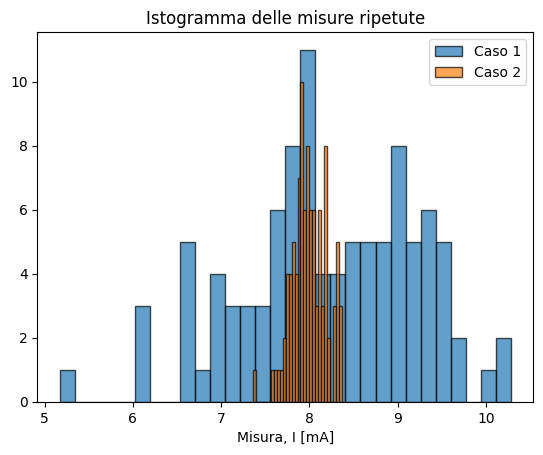
\includegraphics[width=0.8\textwidth]{Immagini/Istogramma.png}
    \caption{Istogramma comparativo delle due serie di misure simulate.}
\end{figure}

\subsection{Propagazione degli Errori}
Data una funzione $f(x,y)$ di variabili casuali indipendenti, la varianza si propaga come:
\begin{equation}
    \sigma_f^2 = \left( \frac{\partial f}{\partial x} \right)^2 \sigma_x^2 + \left( \frac{\partial f}{\partial y} \right)^2 \sigma_y^2
\end{equation}

\begin{example}
\textbf{Esempio numerico:} Calcolo dello spazio percorso in un moto uniformemente accelerato \\
Dati: $v = 200 \pm 10 \, m/s$, \quad $a = 12 \pm 2 \, m/s^2$, \quad $t = 6 \, s$ (errore trascurabile).
\[ s =  vt + \frac{1}{2}at^2 = (200 \cdot 6) + \frac{1}{2} \cdot 12 \cdot 6^2 = 1200 + 216 = 1416 \, m \]

Errore associato $\sigma_s$:
\[ \sigma_s^2 = \left( \frac{\partial s}{\partial v} \right)^2 \sigma_v^2 + \left( \frac{\partial s}{\partial a} \right)^2 \sigma_a^2 = (t)^2 \sigma_v^2 + \left(\frac{1}{2}t^2\right)^2 \sigma_a^2 \]
\[ \sigma_s = \sqrt{ 6^2 \cdot 10^2 + (18)^2 \cdot 2^2 } = \sqrt{3600 + 1296} = \sqrt{4896} \approx 70 \, m \]
Risultato: $s = 1416 \pm 70 \, m$.

\end{example}


\ripasso{Errore di sensibilità e distribuzione uniforme}

Si definisce l'errore di sensibilità come la semiampiezza dell'intervallo di risoluzione: $\displaystyle \Delta x = \frac{X_{\max} - X_{\min}}{N}$. Il risultato della misura sarà espresso come $x \pm \Delta x$.

L'interpretazione statistica assume che il "valore vero" della grandezza appartenga a un insieme continuo di possibili valori $x$, ognuno associato a una probabilità $P(x)$. Poiché nel caso continuo la probabilità di un singolo punto è nulla, si utilizza la \textit{densità di probabilità}, tale che:
\[
P(x_1 < X < x_2) = \int_{x_1}^{x_2} P(x) \; dx
\]
La probabilità totale su tutto il dominio deve essere unitaria (condizione di normalizzazione).

Nel caso continuo, il valore di aspettazione $\mu$ e la varianza $\sigma^2$ sono definiti rispettivamente come il baricentro e il momento di inerzia della distribuzione: $\displaystyle \sigma^2 = \int_{X_{\min}}^{X_{\max}}(x - \mu)^2 P(x) dx$.

Se all'interno dell'intervallo di misura tutti i valori sono \textit{equiprobabili}, $P(x)$ segue una \textbf{distribuzione uniforme}:
\[
P(x)=
\begin{cases}
    c , & x \in [X_{\min}, X_{\max}] \\
    0 , & \text{altrimenti}
\end{cases}
\]

Imponendo la condizione di normalizzazione ($\int P(x)dx = 1$), si ricavano i parametri della distribuzione:
\begin{itemize}
    \item L'altezza della distribuzione è $\displaystyle c = \frac{1}{X_{\max} - X_{\min}}$.
    \item Ponendo per comodità l'origine al centro dell'intervallo (semiampiezza $\Delta$), il valore medio è nullo:
    $\displaystyle \mu = \int_{-\Delta}^{+\Delta} x \frac{1}{2 \Delta } dx = 0$.
    \item La deviazione standard risulta essere:
    $\displaystyle \sigma = \sqrt{\int_{-\Delta}^{+\Delta} (x - 0)^2 \frac{1}{2 \Delta } dx} = \sqrt{\frac{\Delta^2}{3}} = \frac{\Delta}{\sqrt{3}}$.
\end{itemize}

\subsection{Errore di Sensibilità e Distribuzione Uniforme}
Quando non è possibile ripetere molte volte la misura, associamo alle misure l'errore dovuto alla sensibilità dello strumento. Questo errore si ottiene leggendo il minimo scarto della variabile consentito dallo strumento (risoluzione):
\[ \Delta x = \frac{x_{max} - x_{min}}{2} \]
Questo è l'errore massimo $x \pm \Delta x$. Statisticamente, assumere che il valore vero si trovi in $[x_{min}, x_{max}]$ equivale ad assumere una \textbf{densità di probabilità uniforme} $P(x)$ di larghezza $2\Delta$.
La densità deve essere normalizzata a 1:
\[ \int_{-\Delta}^{\Delta} C \, dx = 1 \implies C(2\Delta) = 1 \implies C = \frac{1}{2\Delta} \]

Quindi:
\[ P(x) = \begin{cases} \frac{1}{2\Delta} & x \in [-\Delta, \Delta] \\ 0 & \text{altrove} \end{cases} \]

Per una distribuzione uniforme tra $[-\Delta, \Delta]$:
\begin{itemize}
    \item Media: $\mu = 0$
    \item Varianza: $\sigma^2 = \int_{-\Delta}^{\Delta} x^2 \frac{1}{2\Delta} dx = \frac{\Delta^2}{3}$
\end{itemize}
Quindi, se si vuole convertire un errore massimo $\Delta$ in una deviazione standard $\sigma$:
\begin{equation}
    \sigma = \frac{\Delta}{\sqrt{3}}
\end{equation}

\section{Metodo dei Minimi Quadrati}

\ripasso{Metodo dei Minimi Quadrati}

Un metodo fondamentale per stimare i parametri di un modello è quello dei \textbf{minimi quadrati}. 
Consideriamo un set di misure $\vec{x}=(x_1, \dots, x_n)$ e i corrispondenti valori osservati $\vec{y}=(y_1, \dots, y_n)$. Si assume che esista una relazione funzionale $f(x; \lambda)$ che lega le variabili, dove $\vec{\lambda} = (\lambda_1, \dots, \lambda_k)$ sono i parametri ignoti da stimare.

Il principio dei minimi quadrati stabilisce che la miglior stima dei parametri è quella che minimizza la somma degli scarti quadratici pesati:
\[
\chi^2 = \sum_{i=1}^{n} w_i \left[ y_i - f(x_i; \vec{\lambda}) \right]^2
\]
Il peso $w_i$ è legato all'incertezza della misura:
\begin{itemize}
    \item Se tutte le misure hanno la stessa incertezza, il termine $w_i$ può essere omesso (o posto uguale a 1).
    \item Se ogni misura ha un'incertezza diversa $\sigma_i$, allora $w_i = \frac{1}{\sigma_i^2}$. In questo caso la quantità minimizzata coincide con la variabile $\chi^2$ (Chi-quadro).
    \item Se le variabili sono correlate, i pesi coinvolgeranno gli elementi della matrice di covarianza inversa.
\end{itemize}

\textbf{Caso particolare: stima di una costante (Media Pesata)}
Se il modello è una costante $y = \lambda$ (cioè cerchiamo il miglior valore unico che rappresenti i dati), minimizzando il $\chi^2$ si ottiene:
\begin{itemize}
    \item Con errori uguali ($\sigma_i = \sigma$): Media aritmetica
    \[ \hat{\lambda} = \frac{1}{n} \sum_{i=1}^n y_i \]
    \item Con errori differenti ($\sigma_i$): Media pesata
    \[ \hat{\lambda} = \frac{\sum_{i=1}^n \frac{y_i}{\sigma_i^2}}{\sum_{j=1}^{n}\frac{1}{\sigma_j^2}} \]
\end{itemize}

\subsection{Il Principio}

L'obiettivo è dedurre informazioni fisiche dai dati (fit). Partiamo dalle ipotesi:
\begin{enumerate}
    \item Ho effettuato misure $(x_i, y_i)$ dove l'errore su $x$ è trascurabile.
    \item Per ogni $x$ fisso, ho misurato $y$ con incertezza $\sigma_i$.
    \item Esiste una legge $y = f(x; p)$ (dove $p$ sono i parametri).
\end{enumerate}

Il metodo consiste nel minimizzare la somma degli scarti quadratici pesati, detta \textbf{Chi Quadro} $\chi^2$:
\begin{equation}
    \chi^2 = \sum_{i=1}^{N} \left[ \frac{y_i - f(x_i; p)}{\sigma_i} \right]^2
\end{equation}

Minimizzare significa porre le derivate rispetto ai parametri uguali a zero: $\frac{\partial \chi^2}{\partial p} = 0$.
\ripasso{Fit di una retta (Regressione Lineare)}

Vogliamo determinare la retta che meglio descrive un set di dati $(x_i, y_i \pm \sigma_i)$.
Utilizziamo la parametrizzazione $f(x) = mx + q$ (oppure $\theta_2 x + \theta_1$), dove i parametri da stimare sono la pendenza $m$ e l'intercetta $q$.
Per trovare il minimo, è necessario risolvere il sistema di equazioni ottenuto annullando le derivate parziali del $\chi^2$:
\[ \frac{\partial \chi^2}{\partial m}=0 \quad \text{e} \quad \frac{\partial \chi^2}{\partial q}=0 \]

\subsubsection*{Caso 1: Errori uguali o trascurabili}
Se gli errori $\sigma_i$ sono tutti uguali, la funzione da minimizzare è:
\[
X^2 = \sum_{i=1}^{N} (y_i - q - m x_i)^2
\]
Introducendo i valori medi $\bar{x}, \bar{y}, \overline{x^2}, \overline{xy}$, le soluzioni per i parametri (stimatori) sono:
\[ 
\begin{split}
q &= \hat{\theta}_1 = \frac{\bar{y} \cdot \overline{x^2} - \bar{x} \cdot \overline{xy}}{\overline{x^2} - \bar{x}^2} \\
m &= \hat{\theta}_2 = \frac{\overline{xy} - \bar{x} \cdot \bar{y}}{\overline{x^2} - \bar{x}^2}
\end{split}
\]
Gli errori sui parametri si ricavano dalla legge di propagazione della varianza (assumendo $\sigma_y = \sigma$ costante per tutti i punti):
\[
\sigma_q^2 = \sigma^2 \frac{\overline{x^2}}{N(\overline{x^2}-\bar{x}^2)}
\quad , \quad
\sigma_m^2 = \sigma^2 \frac{1}{N(\overline{x^2}-\bar{x}^2)}
\]
Nota: Il termine al denominatore $(\overline{x^2}-\bar{x}^2)$ è la varianza dei valori $x_i$ del campione.

\textbf{Caso 2: Errori differenti (Fit pesato)}
Quando ogni misura ha un errore $\sigma_i$ diverso, la probabilità di ottenere il set di misure osservato è data dal prodotto delle probabilità (Likelihood):
\[ P(y_1, \ldots, y_N) \propto \prod_{i=1}^N \exp\left( -\frac{(y_i - q - m x_i)^2}{2\sigma_i^2} \right) = \exp\left( -\frac{1}{2} \sum_{i=1}^N \frac{(y_i - q - m x_i)^2}{\sigma_i^2} \right) \]
Massimizzare questa probabilità equivale a minimizzare l'esponente, ovvero il $\chi^2$:
\[ \chi^2 = \sum_{i=1}^N \frac{(y_i - q - m x_i)^2}{\sigma_i^2} \]
Definiamo le seguenti somme pesate per semplificare la notazione:
\[
S = \sum \frac{1}{\sigma_i^2}, \quad S_x = \sum \frac{x_i}{\sigma_i^2}, \quad S_y = \sum \frac{y_i}{\sigma_i^2}, \quad S_{xx} = \sum \frac{x_i^2}{\sigma_i^2}, \quad S_{xy} = \sum \frac{x_i y_i}{\sigma_i^2}
\]
Definiamo inoltre il determinante del sistema come $\Delta = S \cdot S_{xx} - S_x^2$.
Le migliori stime per i parametri sono:
\[
q = \frac{S_{xx} \cdot S_y - S_x \cdot S_{xy}}{\Delta}
\quad , \quad
m = \frac{S \cdot S_{xy} - S_x \cdot S_y}{\Delta}
\]
Le varianze dei parametri, ottenute tramite la propagazione degli errori, sono:
\[
\sigma_q^2 = \frac{S_{xx}}{\Delta}
\quad , \quad
\sigma_m^2 = \frac{S}{\Delta}
\]
Il valore minimo del $\chi^2$ può essere utilizzato per il \textit{test delle ipotesi} (goodness of fit), per verificare se i dati sono compatibili con l'ipotesi lineare.


\subsection{Fit Lineare ($y = mx + q$)}
Nel caso di funzione lineare $f(x) = mx + q$ e $\sigma_i = \sigma$ costanti, risolvendo il sistema delle derivate parziali $\frac{\partial \chi^2}{\partial m} = 0$ e $\frac{\partial \chi^2}{\partial q} = 0$, si ottengono le stime analitiche:

Definiamo le somme:
\[ S_x = \sum x_i, \quad S_y = \sum y_i, \quad S_{xx} = \sum x_i^2, \quad S_{xy} = \sum x_i y_i \]
\[ D = N S_{xx} - (S_x)^2 \]

Le stime dei parametri sono:
\begin{equation}
    m = \frac{N S_{xy} - S_x S_y}{D}, \qquad q = \frac{S_{xx} S_y - S_x S_{xy}}{D}
\end{equation}

E gli errori associati (tramite propagazione):
\begin{equation}
    \sigma_m = \sqrt{\frac{N \sigma^2}{D}}, \qquad \sigma_q = \sqrt{\frac{\sigma^2 S_{xx}}{D}}
\end{equation}

\subsubsection*{Esempio (Fit Lineare)}
\begin{lstlisting}[caption={Fit Lineare dei Minimi Quadrati}]
# Dati simulati: Moto uniforme s = v*t + s0
t = np.array([0, 1, 2, 3, 4, 5])       # Tempo [s]
s = np.array([2, 17, 27, 37, 47, 63])  # Spazio [mm]
sigma_s = 2                            # Incertezza [mm]
N = len(t)

# Calcolo Somme
Sx = np.sum(t); Sy = np.sum(s)
Sxx = np.sum(t**2); Sxy = np.sum(t * s)

# Calcolo Parametri
D = N * Sxx - Sx**2
m = (N * Sxy - Sx * Sy) / D
q = (Sxx * Sy - Sx * Sxy) / D

print(f"Velocita' (m): {m:.2f} mm/s")
print(f"Posizione init (q): {q:.2f} mm")

# Plot
plt.errorbar(t, s, yerr=sigma_s, fmt='o', label='Dati')
plt.plot(t, m*t + q, label='Fit Lineare')
plt.xlabel('Tempo [s]'); plt.ylabel('Spazio [mm]')
plt.legend(); plt.show()
\end{lstlisting}


\begin{figure}[H]
    \centering
    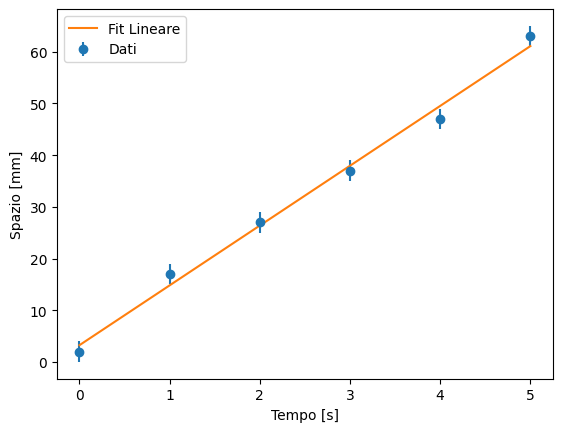
\includegraphics[width=0.8\textwidth]{Immagini/Fit Lineare.png}
    \caption{Fit Lineare}
\end{figure}



\ripasso{Caso non lineare}
Se la relazione tra le grandezze non è lineare, spesso è possibile "linearizzare" il problema con un cambio di variabile.

\begin{example}
    Consideriamo la legge del moto: $s = \frac{1}{2} g t^2$. 
    Supponiamo di voler misurare $g$ trascurando l'incertezza su $s$ e considerando solo l'errore su $t$.
    Possiamo riscrivere l'equazione come:
    \[ t = \sqrt{\frac{2}{g}} \sqrt{s} \]
    Ponendo $y = t$, $x = \sqrt{s}$ e il parametro $m = \sqrt{\frac{2}{g}}$, otteniamo una relazione lineare $y = mx$ (con intercetta nulla).
    
    Una volta stimato $m$ e la sua varianza $\sigma_m^2$ con il metodo dei minimi quadrati, ricaviamo $g$ invertendo la relazione: $g = \frac{2}{m^2}$.
    L'errore su $g$ si ottiene con la propagazione:
    \[
    \sigma_g = \left| \frac{\partial g}{\partial m} \right| \sigma_m = \left| -\frac{4}{m^3} \right| \sigma_m
    \]
    Questo esempio evidenzia l'importanza della scelta delle variabili dipendenti e indipendenti.
\end{example}

Nei casi in cui la linearizzazione non è possibile, si ricorre all'espansione di Taylor del modello attorno a valori iniziali dei parametri o a metodi numerici iterativi.
\subsection{Caso Non Lineare e Linearizzazione}
se $f(x; p)$ non è lineare spesso si cerca un'espressione linearizzata cambiando variabili.
\\
\\
\textbf{Esempio:} Caduta grave $h = \frac{1}{2}g t^2$ oppure la formula inversa per calcolare $g$ dai tempi:
\[ t = \sqrt{\frac{2}{g}}\sqrt{d} + t_0 \]
Questa equazione è del tipo $Y = mX + q$ se poniamo:
\[ Y = t, \quad X = \sqrt{d}, \quad m = \sqrt{\frac{2}{g}}, \quad q = t_0 \]

Una volta calcolato $\hat{m}$ con i minimi quadrati, inverto la relazione per trovare $g$:
\[ \hat{m}^2 = \frac{2}{g} \implies g = \frac{2}{\hat{m}^2} \]
Per l'errore, uso la propagazione:
\[ \sigma_g = \left| \frac{\partial g}{\partial m} \right| \sigma_m = \left| - \frac{4}{m^3} \right| \sigma_m \]

\subsubsection*{Esempio Computazionale (Linearizzazione)}
\begin{lstlisting}[caption={Linearizzazione per calcolo di g}]
# Dati: Tempo t vs Spazio s
t = np.array([0.16, 0.40, 0.58, 0.72, 0.97]) 
s = np.array([0.20, 1.0, 2.0, 3.0, 5.0])
rad_s = np.sqrt(s) # Variabile linearizzata X

# ... (Codice per calcolo m e q su t vs rad_s omesso per brevita'...)
# Supponiamo m sia stato calcolato:
m_calc = 0.45 
sigma_m = 0.01

# Calcolo fisico
g = 2 / m_calc**2
sigma_g = (4 / m_calc**3) * sigma_m

print(f"g misurato: {g:.2f} +/- {sigma_g:.2f} m/s^2")
\end{lstlisting}




\lezione{Momenti e Distribuzioni}{23 Febbraio 2025}



\subsection{Momenti della funzione di distribuzione}



Il valore di aspettazione e la varianza di una variabile casuale sono due particolari “momenti” della funzione densità di probabilità $f_X(x)$.

Possiamo distinguere tra momenti calcolati rispetto all’origine e momenti calcolati rispetto al valore di aspettazione (la media). In entrambi i casi, si tratta di valori di aspettazione (dunque quantità numeriche) delle potenze di $x$ o di $x-\mu_x$. 
Nello specifico definiamo: Il 
Nello specifico, definiamo:
\begin{itemize}
    \item \textbf{Momento algebrico di ordine k} (o k-esimo momento algebrico): calcolato rispetto all'origine.
    \item \textbf{Momento centrale di ordine k}: calcolato rispetto alla media.
\end{itemize}

Le formule sono rispettivamente:
\[
\mu_k^* = E[x^k] \qquad \mu_k =E[{(x - \mu_x)}^k]
\]

Di conseguenza $\mu$ non è altro che il momento di ordine 1 rispetto all'origine, mentre $\sigma^2$ è il momento di ordine 2 rispetto alla media.

I momenti sono fondamentali perché caratterizzano interamente le funzioni di distribuzione: sotto ipotesi non particolarmente restrittive, si può affermare che due funzioni aventi gli stessi momenti coincidono.


\subsection{Distribuzione uniforme discreta}
Consideriamo una variabile $X$ che può assumere $n$ valori discreti. Se tutti i valori sono equiprobabili, imponendo la condizione di normalizzazione si ottiene che la probabilità per ogni valore è $p=1/n$.
Di conseguenza, il valore medio è:
\[
\mu_x=\frac{1}{n}\sum_{i=1}^{n}x_i
\]
che corrisponde alla media aritmetica dei possibili valori (analogo al lancio di un dado).
La varianza è data da:
\[
{\sigma_x}^2=\frac{1}{n} \sum_{i=1}^{n}(x_i-\mu_x)^2
\]


\subsection{Distribuzione uniforme continua}
Una variabile casuale continua definita nell'intervallo $(a,b)$ possiede una distribuzione uniforme se la sua densità di probabilità è costante, ovvero $f_X(x) = \text{cost}$.
Affinché sia soddisfatta la condizione di normalizzazione (l'area sotto la curva deve essere 1), la funzione deve essere:
\[
f_X(x)=\frac{1}{b-a}
\]

Il valore medio si calcola come:
\[
\mu_x=\int_{a}^{b}x f(x) dx = \frac{a+b}{2}
\]


Per la varianza, sfruttando la proprietà $E[x^2]-{E[x]}^2$, si ottiene:
\[
{\sigma_x}^2 = \frac{{(b-a)^2}}{12}
\]


\begin{nota}
    \textbf{Collegamento con la trattazione degli errori.} \\
    Quando si passa dalla teoria degli errori massimi a quella statistica, il risultato di una misura viene espresso come $x \pm \Delta x$. Questo intervallo corrisponde a una distribuzione uniforme di larghezza $b-a = 2\Delta x$.

    Sostituendo nella formula della varianza ricavata sopra ($\sigma_x^2=\frac{(b-a)^2}{12}$), otteniamo la deviazione standard:
    \[
    \sigma_x=\frac{b-a}{2\sqrt{3}} \quad \Rightarrow \quad \Delta x = \sigma_x \sqrt{3}
    \]
    È interessante calcolare la probabilità che il valore $x$ cada all'interno dell'intervallo di una deviazione standard dalla media ($\mu_x \pm \sigma_x$). Tale probabilità risulta essere:
    \[
    P(\mu_x-\sigma_x < x \leq \mu_x + \sigma_x) = \frac{1}{\sqrt{3}} \approx 0.577
    \]
    
    \textit{Dimostrazione:}
    \[
    \int_{\mu_x-\sigma_x}^{\mu_x+\sigma_x} f(x)dx = \frac{1}{b-a}\int_{\mu_x-\sigma_x}^{\mu_x+\sigma_x} dx = \frac{1}{b-a} (2 \sigma_x) = \frac{2\sigma_x}{2\sigma_x\sqrt{3}} = \frac{1}{\sqrt{3}}
    \]
\end{nota}

\vspace{1 cm}

\begin{definizione}
\textbf{Momenti di ordine k}: 
\[
\mu_k=E[x^k]=\int_\Omega x^k f(x) dx
\]
\end{definizione}

\textbf{Osservazioni:}
\begin{itemize}
    \item Per $k=0 \quad \to \quad  \mu_0 =\int_\Omega f(x) dx =1$ (Normalizzazione della funzione di probabilità).
    \item Per $k=1 \quad \to \quad \mu_1$ rappresenta il valore di aspettazione o media (il baricentro della distribuzione).
\end{itemize}

\begin{definizione}
\textbf{Momenti centrali di ordine k}:
\[
\bar{\mu}_k=E[(x-\mu)^k]=\int_\Omega (x-\mu)^k f(x) dx
\]
\end{definizione}

\textbf{Osservazione:}
\begin{itemize}
    \item Per $k=0 \quad \to \quad \bar{\mu}_0= \int_\Omega f(x) dx = 1$.
    \item Per $k=1 \quad \to \quad \bar{\mu}_1= 0$. \\
    \textit{Dimostrazione:} $\int_\Omega (x-\mu)f(x) dx = \int_\Omega x f(x) dx - \mu \int_\Omega f(x) dx = \mu - \mu \cdot 1 = 0$.
    \item Per $k=2 \quad \to \quad \bar{\mu}_2=\sigma^2$ (Varianza).
    \item Per $k=3 \quad \to \quad \bar{\mu}_3$ è legato all'\textit{indice di asimmetria} (o \textit{skewness}). Esso indica quanto la distribuzione sia simmetrica rispetto alla media:
    \pgfplotsset{
        skewplot/.style={
            width=8cm, height=4cm, 
            axis lines=left,
            xtick=\empty, ytick=\empty, 
            xlabel={$x$},
            ymin=0,
            no markers,
            axis line style={-},
            hide y axis 
        }
    }
    \begin{itemize}
        \item per una distribuzione simmetrica (es. Gaussiana) $\bar{\mu}_3=0$;
         
        \begin{center}
        \begin{tikzpicture}
            \begin{axis}[skewplot, title={Simmetrica ($\bar{\mu}_3=0$)}]
                % Gaussiana
                \addplot[domain=-3:3, samples=60, smooth, thick, RoyalBlue, fill=RoyalBlue!10] {exp(-x^2/2)} \closedcycle;
                % Linea della media
                \draw[dashed, black] (axis cs:0,0) -- (axis cs:0,1) node[above, font=\tiny] {$\mu$};
            \end{axis}
        \end{tikzpicture}
        \end{center}

        \item per una distribuzione asimmetrica a destra (es. Maxwell-Boltzmann) $\bar{\mu}_3>0$;
         \begin{center}
        \begin{tikzpicture}
            \begin{axis}[skewplot, title={Asimmetrica a destra ($\bar{\mu}_3>0$)}]
                % Funzione con coda a destra (simile a Gamma)
                \addplot[domain=0:8, samples=80, smooth, thick, RoyalBlue, fill=RoyalBlue!10] {x^1.8 * exp(-x)} \closedcycle;
                % Nota: Coda lunga verso i valori positivi (destra)
            \end{axis}
        \end{tikzpicture}
        \end{center}

        \item per una distribuzione asimmetrica a sinistra $\bar{\mu}_3<0$
    \begin{center}
        \begin{tikzpicture}
            \begin{axis}[skewplot, title={Asimmetrica a sinistra ($\bar{\mu}_3<0$)}]
                % Speculare alla precedente (coda a sinistra)
                \addplot[domain=-8:0, samples=80, smooth, thick, RoyalBlue, fill=RoyalBlue!10] {(-x)^1.8 * exp(-(-x))} \closedcycle;
                % Nota: Coda lunga verso i valori negativi (sinistra)
            \end{axis}
        \end{tikzpicture}
        \end{center}

    \end{itemize}     

        \item Per $k=4 \quad \to \quad \bar{\mu}_4$ è legato all'\textit{indice di curtosi} (o \textit{kurtosis}). Questo parametro valuta il peso delle "code" della distribuzione, ovvero l'influenza dei valori estremi (\textit{outliers}).

\end{itemize}
\vspace{1 cm}
L'introduzione dei momenti risulta utile per diversi motivi. Un risultato fondamentale è il seguente: se due variabili casuali $X$ e $Y$ possiedono gli stessi momenti, allora le loro funzioni di distribuzione di probabilità ($f_X$ e $f_Y$) sono identiche.

\begin{definizione}
    \textbf{Funzione generatrice dei momenti}:
        La funzione generatrice dei momenti, indicata con $M_x(t)$, è definita come il valore atteso di $e^{tx}$. La sua espressione varia a seconda che la variabile casuale sia continua o discreta:
    \[
    M_x(t) = E[e^{tx}] = 
    \begin{cases} 
    \displaystyle \int_\Omega e^{tx}f(x) dx & \text{caso continuo} \\[1em]
    \displaystyle \sum_i p_i e^{tx_i} & \text{caso discreto}
    \end{cases}
    \]
\end{definizione}
Questa funzione è fondamentale perché permette di "generare" i momenti della distribuzione (come media, varianza, ecc.) attraverso l'operazione di derivazione. Calcolando la derivata $m$-esima rispetto a $t$ e valutandola in $t=0$, si ottiene il momento $m$-esimo semplice:

\[
\left[ \frac{\partial ^m M_x}{\partial t^m} \right]_{t=0} = E[x^m] = \mu_m
\]

\paragraph{Dimostrazione:}
Per dimostrare questa proprietà, sviluppiamo $e^{tx}$ in serie di Maclaurin:
\[ 
e^{tx} = \sum_{k=0}^{\infty} \frac{(tx)^k}{k!} 
\]
Sostituendo questo sviluppo nell'integrale della definizione (assumendo il caso continuo per generalità) e sfruttando la linearità dell'integrale, otteniamo:
\[
M_x(t) = \int_\Omega \left( \sum_{k=0}^{\infty} \frac{(tx)^k}{k!} \right) f(x) dx = \sum_{k=0}^{\infty} \frac{t^k}{k!} \int_\Omega x^k f(x) dx 
\]
Poiché l'integrale $\int_\Omega x^k f(x) dx$ corrisponde esattamente al momento $k$-esimo $\mu_k$, possiamo scrivere:
\[
M_x(t) = \sum_{k=0}^{\infty} \frac{t^k}{k!} \mu_k = \mu_0 + \mu_1 t + \frac{\mu_2 t^2}{2!} + \ldots
\]
Se calcoliamo la derivata prima rispetto a $t$:
\[ \frac{\partial M_x}{\partial t} = \mu_1 + \frac{2\mu_2 t}{2!} + \ldots = \mu_1 + \mu_2 t + \ldots \]
Ponendo $t=0$, tutti i termini con $t$ si annullano, lasciando solo il coefficiente $\mu_1$:
\[ \left[ \frac{\partial M_x}{\partial t} \right]_{t=0} = \mu_1 = E[x] \]

\begin{definizione}
    \textbf{Funzione generatrice dei momenti centrali}:
    Analogamente, è possibile definire la funzione che genera i momenti rispetto alla media $\mu$ (momenti centrali):
        \[
    \bar{M}_x(t) = E[e^{t(x-\mu)}] = 
    \begin{cases} 
    \displaystyle \int_\Omega e^{t(x-\mu)}f(x) dx & \text{caso continuo} \\[1em]
    \displaystyle \sum_i p_i e^{t(x-\mu_i)} & \text{caso discreto}
    \end{cases}
    \]
\end{definizione}

Anche in questo caso vale la proprietà delle derivate:
\[
\left[ \frac{\partial ^m \bar{M}_x}{\partial t^m}\right]_{t=0} = E[(x-\mu)^m] = \bar{\mu}_m 
\]


Esiste una relazione diretta tra la funzione generatrice dei momenti semplici e quella dei momenti centrali. Sfruttando le proprietà dell'esponenziale e la linearità del valore atteso, si ha:
\[
\bar{M}_x(t) = E[e^{t(x-\mu)}] = E[e^{tx}e^{-t\mu}] = e^{-t\mu}E[e^{tx}] = e^{-t\mu}M_x(t)
\]


Infine se due variabili casuali $X$ e $Y$ possiedono la stessa funzione generatrice dei momenti ($M_x(t)=M_y(t)$) o la stessa funzione generatrice dei momenti centrali ($\bar{M}_x(t)=\bar{M}_y(t)$), allora le loro distribuzioni di probabilità ($f_X$ e $f_Y$) sono identiche.

\begin{definizione}
    \textbf{Funzione caratteristica}:
    Una variante importante è la funzione caratteristica, definita come:
    \[
    \phi (x) = E[e^{itx}] = \int_\Omega e^{itx}f(x) dx
    \]
    Questa corrisponde formalmente alla \textbf{Trasformata di Fourier} della densità di probabilità.
\end{definizione}
Consideriamo una variabile aleatoria $Z = X + Y$, somma di due variabili aleatorie \textbf{indipendenti} $X$ e $Y$.
La funzione generatrice dei momenti della somma è il prodotto delle singole funzioni generatrici:
\[
M_Z(t) = E[e^{tZ}] = E[e^{t(X+Y)}] = E[e^{tX}e^{tY}]
\]
Essendo $X$ e $Y$ indipendenti, il valore atteso del prodotto è il prodotto dei valori attesi:
\[
M_Z(t) = E[e^{tX}]E[e^{tY}] = M_X(t)M_Y(t)
\]


\subsection{Distribuzione binomiale o di Bernoulli}
\emph{Questa parte è stata integrata con gli appunti di Bressan}
\vspace{0.4 cm}

La distribuzione binomiale descrive un fenomeno che può verificarsi solo con due modalità mutualmente esclusive: successo (con probabilità $p$) o insuccesso (con probabilità $q=1-p$).

Se ripetiamo l'esperimento $n$ volte, la probabilità di ottenere esattamente $k$ successi è data dalla funzione:
\[
P(k;n,p) = \binom{n}{k}p^k q^{n-k} = \frac{n!}{k!(n-k)!}p^k (1-p)^{n-k}
\]
Casi particolari immediati:
\begin{itemize}[itemsep=0.1em]
 \item Probabilità di $n$ successi (tutti): $p^n$ 
 \item Probabilità di $0$ successi (nessuno): $q^n$  
 \item Probabilità di $1$ successo: $n p q^{n-1}$ (nota: il coefficiente binomiale $\binom{n}{1}=n$)
 \item Probabilità di $n-1$ successi: $n p^{n-1}q$
\end{itemize}

\begin{example}
    Consideriamo 3 oggetti ($n=3$) chiamati A, B, C. Vogliamo sceglierne 2 ($k=2$). 
    Le possibili combinazioni sono: AB, BC, AC.
    Calcolando con la formula del coefficiente binomiale otteniamo conferma:
    \[
    \binom{3}{2} = \frac{3!}{2!(3-2)!} = \frac{3 \cdot 2 \cdot 1}{2 \cdot 1 \cdot 1} = 3
    \]
\end{example}

\subsubsection{Proprietà della distribuzione binomiale}
\begin{itemize}
    \item \textbf{Normalizzazione}: La somma di tutte le probabilità è 1. Questo deriva dallo sviluppo del binomio di Newton:
    \[ \sum_{k=0}^{n} \binom {n}{k}p^kq^{n-k} = (p+q)^n = (1)^n = 1 \]
    
    \item \textbf{Calcolo diretto della media}: Possiamo derivare la media manipolando la sommatoria. Derivando l'identità $(p+q)^n$ rispetto a $p$:
    \[
    p \frac{\partial}{\partial p} (p + q)^n = p \cdot n(p+q)^{n-1} \quad \xrightarrow{p+q=1} \quad np
    \]
    Dall'altro lato della sommatoria:
    \[
    p \frac{\partial}{\partial p} \sum_{k=0}^{n} \binom{n}{k} p^k q^{n-k} = \sum_{k=0}^{n} k \binom{n}{k} p^k p^{-1} q^{n-k} \cdot p = \sum_{k=0}^{n} k \binom{n}{k} p^k q^{n-k} = E[k]
    \]
    Uguagliando i risultati otteniamo il valore atteso: $E[k] = np$.
    
    \item \textbf{Varianza}: La varianza è data da $\sigma_x^2 = E[x^2] - E[x]^2 = npq$.
\end{itemize}

\subsubsection{Funzione generatrice dei momenti della Binomiale}
Calcoliamo il momento generatore per la binomiale:
\[
M_k(t) = E[e^{tk}] = \sum_{k=0}^{n} e^{tk} \binom{n}{k} p^k q^{n-k} = \sum_{k=0}^{n} \binom{n}{k} (pe^t)^k q^{n-k}
\]
Riconoscendo la forma del binomio di Newton $(a+b)^n$ con $a=pe^t$ e $b=q$, otteniamo:
\[
M_k(t) = (pe^t + q)^n
\]

Da qui possiamo ricalcolare i momenti derivando rispetto a $t$:

\begin{enumerate}
    \item \textbf{Valore atteso (Media)}:
    Calcoliamo la derivata prima:
    \[ M'_k(t) = n(pe^t+q)^{n-1} \cdot pe^t \]
    Ponendo $t=0$ (ricordando che $e^0=1$ e $p+q=1$):
    \[ \mu = M'_k(0) = n(p+q)^{n-1}p = np \]

    \item \textbf{Varianza}:
    Calcoliamo la derivata seconda (regola del prodotto):
    \[ M''_k(t) = n(n-1)(pe^t+q)^{n-2}(pe^t)^2 + n(pe^t+q)^{n-1}pe^t \]
    Ponendo $t=0$:
    \[ E[x^2] = M''_k(0) = n(n-1)p^2 + np \]
    Ora calcoliamo la varianza usando $Var(x) = E[x^2] - E[x]^2$:
    \[
    \sigma^2 = [n(n-1)p^2 + np] - (np)^2 = n^2p^2 - np^2 + np - n^2p^2 = np - np^2 = np(1-p) = npq
    \]

    \item \textbf{Asimmetria (Terzo momento centrale)}:
    Il terzo momento centrale è $\bar{\mu_3} = npq(1-2p)$. Questo indice ci dice la forma della distribuzione:
    \begin{itemize}
        \item Se $\bar{\mu_3} > 0$: distribuzione \textbf{asimmetrica positiva} (coda a destra).
        \item Se $\bar{\mu_3} = 0$: distribuzione \textbf{simmetrica}.
        \item Se $\bar{\mu_3} < 0$: distribuzione \textbf{asimmetrica negativa} (coda a sinistra).
    \end{itemize}
\end{enumerate}

\vspace{0.5cm}

\paragraph{Limiti della Binomiale:}
La distribuzione binomiale è estremamente importante in fisica perché, al limite per $n \to \infty$, approssima altre distribuzioni fondamentali:
\begin{itemize}
    \item Tende alla \textbf{distribuzione di Gauss} se $p$ rimane costante.
    \item Tende alla \textbf{distribuzione di Poisson} se il prodotto $np$ rimane costante (ovvero se $p \to 0$ mentre $n \to \infty$).
\end{itemize}

\paragraph{Applicazione agli istogrammi:}
Consideriamo un istogramma dove $n$ è il numero totale di eventi e ci focalizziamo su un particolare intervallo (bin) $i$.
Il numero atteso di eventi in quell'intervallo è $E[n_i] = n p_i$.

La varianza del numero di eventi nell'intervallo è data dalla binomiale:
\[ \sigma_{n_i}^2 = n p_i (1 - p_i) = n_i (1 - p_i) \simeq n_i \left(1 - \frac{n_i}{n}\right) \]
Se stimiamo la probabilità $p_i$ tramite i dati misurati come $\hat{p_i} = n_i^{mis}/n$, nel caso in cui la probabilità sia molto piccola ($p \to 0$, regime di Poisson), il termine $(1-p_i) \approx 1$.
Di conseguenza, l'errore standard (deviazione standard) sul conteggio di un bin è approssimabile con la radice quadrata del conteggio stesso:
\[ \sigma_{n_i} \approx \sqrt{n_i^{mis}} \]

\lezione{Codice python e Distribuizione di Poisson}{26 Febbraio 2025}

\subsection{Esempi python}
aggiungi l'Esercizio che ha messo su python (lancio della moneta)



\subsection{Distribuzione di Poisson}
La distribuzione di Poisson è un caso limite della distribuzione binomiale, che si ottiene quando il numero di prove $n$ tende all'infinito e la probabilità di successo $p$ tende a zero, mantenendo costante il prodotto $np = \mu$ (dove $\mu$ rappresenta il valore atteso).
si usa nei casi in cui si voglia indicare la probabilità di osservare $k$ eventi in un intervallo di tempo $t$ se si fanno un numero fissato di tentativi.
La poissoniana si applica in cui ho un particolare risultato ma non ha senso di parlare del "non risultato".
Per esempio il numero di fulmini che cadono in un certo intervallo di tempo, o il numero di particelle che attraversano una certa area in un certo intervallo di tempo e non esiste un "non evento" (non posso avere un fulmine che cade e non cade contemporaneamente).
Il processo non ha memeoria, un evento che si è verificato non influenza la probabilità che si verifichi un altro evento in futuro.

\[ \lim_{n \to \infty; p \to 0}  Bin / \lambda = np = cost \]

 lambda eventi in un certo $\Delta t$ in media (frequenza), posso dividere $\Delta t$ in intervallini  di tempo $\Delta t'$ in modo che in ogni suddivisione accada al massimo un solo evento  
avrò $P= \frac{\lambda}{n}$ ovvero la probabilità di avere un evento (dove n è iul numero di intervalli e  $\lambda$ è il numero medio di ).  

Quindi la probabilità di avere k eventi in un intervallo di tempo t è data dalla binomiale:
\[ P(k; n,\frac{\lambda}{n}) = \frac{\lambda^k}{n^k} (1- \frac{\lambda}{n})^{n-k} \frac{n!}{k!(n-k)!} \] 

passiamo per il limite $n \to \infty$ e otteniamo la formula della distribuzione di Poisson:
\[
\frac{n!}{(n-k)!} = \frac{n (n-1) \cdots (n-k+1) (n-k)!}{(n-k)!} \to_{n \to \infty} n^k
\]

un esempio con k=5:
\[ 
\frac{n!}{(n-5)!} = \frac{n(n-1)(n-2)(n-3)(n-4)}{1} \to_{n \to \infty} n^5
\]

poi:

\[
(1-\frac{\lambda}{n})^k \to_{n \to \infty} (1- \frac{\lambda}{k})^n \to_{n \to \infty} e^{-\lambda}
\]

Quindi si trova che:
\[ P(k; n,\frac{\lambda}{n}) \to_{n \to \infty} \frac{\lambda^k}{k!} e^{-\lambda} \]

Quale è la probabili di osservare K eventi sapendo che la media è $\lambda$ e $0 \leq k \leq \infty$.
Il decadimento radiattivo è un esempio classico di processo che segue una distribuzione di Poisson, in quanto il numero di decadimenti in un intervallo di tempo è discreto.

Ora calcoliamo il valore di aspettazione e variazioni standard con le funzioni generatrici dei momenti:
\[
M_k(t) = E[e^{tk}] = \sum_{k=0}^{\infty} e^{tk} \frac{\lambda^k}{k!} e^{-\lambda} = e^{-\lambda} \sum_{k=0}^{\infty} \frac{(\lambda e^t)^k}{k!} = e^{-\lambda} e^{\lambda e^t} = e^{\lambda(e^t - 1)} \]

dove abbiamo usato lo sviluppo di Taylor dell'esponenziale per riconoscere la serie come $e^{\lambda e^t}$ $\left( e^x = \sum_{k=0}^{\infty} \frac{x^k}{k!} \right)$.
\\
\\
Calcoliamo la derivata prima per ottenere il valore di aspettazione:
\[ M'_k(t) = \lambda e^t e^{\lambda(e^t - 1)} \quad \Rightarrow \quad M'_k(0) = \lambda e^0 e^{\lambda(e^0 - 1)} = \lambda \]
Calcoliamo la derivata seconda per ottenere $E[k^2]$:
\[ M''_k(t) = \lambda e^t e^{\lambda(e^t - 1)} + \lambda^2 e^{2t} e^{\lambda(e^t - 1)} \]
\[ M''_k(0) = \lambda + \lambda^2 = \lambda(1 + \lambda) \]
Quindi:
\[ E[k^2] = M''_k(0) = \lambda(1 + \lambda) \]
E la varianza è:
\[ {\sigma^2} = E[k^2] - (E[k])^2 = \lambda(1 + \lambda) - \lambda^2 = \lambda \]

La funzione generatrice dei momenti permette alternativamente di verificare che la Poissoniana coincide con il limite della binomiale:

\[ Bin \to M_k(t) = (pe^t + q)^n  = (pe^t + 1-p)^n = (1+ \frac{\lambda}{n}(e^t -1))^n 
\]
Passiamo al limite:
\[ 
\lim_{n \to \infty} M_k(t) = \lim_{n \to \infty} (1+ \frac{\lambda}{n}(e^t -1))^n = e^{\lambda(e^t - 1)}
\]
che è proprio la funzione generatrice dei momenti della distribuzione di Poisson, confermando così la connessione tra le due distribuzioni.

\textbf{Osservazioni}
\begin{itemize}
    \item 
La poissoniana ha code più lunghe perché è più probabile osservare valori lontani dalla media rispetto alla binomiale, soprattutto quando la media è piccola. Questo è dovuto al fatto che la poissoniana è un limite della binomiale in cui il numero di prove tende all'infinito e la probabilità di successo tende a zero, mantenendo costante il prodotto $np$. In questo regime, la distribuzione si concentra su valori piccoli di $k$, ma non esclude completamente la possibilità di osservare valori più grandi, dando luogo a code più lunghe rispetto alla binomiale.
un'altra cosa è che la varianza della binomiale è $npq$ mentre quella della poissoniana è $np$ (ovvero $npq$ con $q=1$), quindi la poissoniana ha una varianza più grande rispetto alla binomiale, contribuendo ulteriormente alla presenza di code più lunghe.

\[ 
npq = np(1-p) = np -np^2 < np = \lambda 
\]
si vede che la varianza della binomiale è sempre minore di quella della poissoniana, confermando così che la poissoniana ha code più lunghe rispetto alla binomiale.

\item 
si prendano 2 fenomeni descritti da distribuzioni Poisson con rispettivamente $\lambda_a; \lambda_b$, sappiamo che $K=K_a+K_b$ (ovvero che i processi non si possono distinguere) e che $K_a$ e $K_b$ sono indipendenti, quindi la funzione generatrice dei momenti di K è il prodotto delle funzioni generatrici dei momenti di $K_a$ e $K_b$:
infatti valutando la probabilità $P(K_a + K_b, \lambda_a,\lambda_b)$  si trova che p ancora Poissoniana.

prendendo i momenti generatori di una poissoniana:
\[
M_{a+b} (t) = M_a(t) \cdot M_b(t) = e^{\lambda_a(e^t - 1)} \cdot e^{\lambda_b(e^t - 1)} = e^{(\lambda_a + \lambda_b)(e^t - 1)} = e^{\lambda(e^t - 1)}
\]

\end{itemize}

Aggiungere esempi python (notte san Lorenzo, poissoniane ecc).

\subsection{rappresentazione grafica}
se ho un set di dati $N \to {x_1,x_2,...,x_N}$ posso rappresentare la distribuzione di probabilità con un istogramma, che è una rappresentazione grafica che mostra la frequenza o la probabilità di occorrenza di diversi intervalli di valori (bin) all'interno del set di dati.
se le variabili sono descritti da una certa $P(x)$ la probabilità $p_i$ che cada in un certo bin $i$ è data da:
\[
p_i = \int_{x_i}^{x_i+\Delta x} P(x) dx \simeq P(x_i)\Delta x
\]

se indico con $n_i$ il numero di eventi che cadono nel bin $i$, allora $n_i \simeq$ Binomiale$(N, p_i)$ dove $N$ è il numero totale di eventi e $p_i$ è la probabilità che un evento cada nel bin $i$.
quindui vuol dire che il valore di aspettazione:
\[ E[n_i] = N p_i \simeq N \cdot P(x_i) \Delta x \]

\newpage
\section{Parte di Bressan da integrare dopo}
\subsection{Distribuzione di Poisson}
È un caso limite della fisica nucleare, e serve per indicare la probabilità di osservare k eventi in un determianto intervallo t:
\begin{itemize}
    \item la presenza/assenza dell'evento non dipende da quelli prima di t
    \item la probabilità di un evento è proporzionale a t
    \item la probabilità di avere due eventi contemporaneamente è nulla
\end{itemize}
Si tratta del caso in cui i successi $p$ della binomiale siano piccoli e il numero di eventi $n \rightarrow \infty$. 
\[
    P_k(t)=\frac{(\mu t)^k}{k!}e^{\mu t}
\]
La probabilità di avere 0 eventi in (o,t +dt):
\[
P_0(t+dt)=P_0(t)(1-\mu dt) \rightarrow P_0(t)=e^{-\mu t}
\]
dove ho impostato che $P_0(0)=1$ e sottrago $\mu dt$ che è la probabilità di avere un evento in $dt$ ($e^{-\mu dt}\simeq 1-\mu dt$ tolgo il termine quadratico risultante)

La probabilità di avere un evento è invece:
\[
P_1(t+dt)=P_1(1-\mu dt) + P_0(\mu dt) \rightarrow \frac{dP_1}{dt}=- \mu (p_1(t)-p_0(t))
\]

Continuando in maniera ricorsiva trovo che la probabilità di avere "m" eventi in un determinato intervallo è:
\[
\frac{dP_m}{dt}=- \mu (p_m(t)-p_{m-1}(t))
\]
che ha come soluzione:
\[
P_k(t)=\frac{(\mu t)^k}{k!}e^{\mu t}=\frac{(m)^k}{k!}e^{m}
\]
dove $m=\mu t=E[k]$ mi rappresenta il valore di aspettazione di un certo k

La distribuzione di Poisson naturalmente è normalizzata (ricordando lo sviluppo di Taylor dell'esponenziale), infatti:
\[
\sum_{K=0}^{\infty}P_k=e^{-m} \sum_{k=0}^{\infty}\frac{m^k}{k!}=1
\]
e il valore di aspettazione non è altro che:
\[
E[k]=\sum_{k=0}^{\infty}k P_k = m 
\]
e la varianza è:
\[
{\sigma^2}=E[k^2]-{E[k]}^2=m
\]

Si può notare che la distribuzione di Poisson non è altro che il limite per $n \rightarrow \infty$ della distribuzione di Bernulli.


\subsection{Distribuzione di Maxwell-Boltzmann}

Si considera un gas con peso molare \( M = N_A m \) in equilibrio termodinamico a temperatura \( T \). La costante dei gas è \( R = N_A k \approx 8.31 \, \text{J} \, \text{K}^{-1} \text{mol}^{-1} \).

La velocità quadratica media delle molecole del gas è legata alla temperatura dalla relazione:
    \[
    v_{\text{qm}} = \sqrt{\langle v^2 \rangle} = \sqrt{\frac{3RT}{M}}
    \]
    Tuttavia, le singole molecole hanno velocità che si discostano da questo valore medio.

Maxwell nel 1859 derivò la distribuzione di probabilità delle velocità \( f(v) \):
    \[
    f(v) = 4\pi \left( \frac{M}{2\pi RT} \right)^{3/2} v^2 \exp \left[ -\frac{Mv^2}{2RT} \right] = 4\pi \left( \frac{m}{2\pi kT} \right)^{3/2} v^2 \exp \left[ -\frac{mv^2}{2kT} \right]
    \]

    All'aumentare della temperatura, il picco della distribuzione (velocità più probabile) si sposta verso valori più elevati.

Le curve sono normalizzate in modo che l'integrale della probabilità sia sempre uguale a 1.

La distribuzione fu ottenuta da Maxwell attraverso un ragionamento particolarmente ingegnoso:
\begin{itemize}
    \item introduciamo prima alcune definizioni:
    \begin{align*}
        \rho(\vec{r}) &= \frac{dm}{dV} \quad \text{densità del gas}, \\[6pt]
        \eta(\vec{r}) &= \frac{\rho(\vec{r})}{m} \quad \text{densità di particelle}, \\[6pt]
        dn &= \eta(\vec{r}) \, dV \quad \text{numero di particelle in } dV.
    \end{align*}
    \item da cui ricaviamo che la distribuzione delle particelle nello spazio è:
    \[ p(\vec{r})=\frac{\eta (\vec{r})}{n_T}\]
    \item introduciamo una densità di particelle nello spazio delle velocità, in modo analogo a quello tridimensionale: \[ dn(\vec{v})=\eta (\vec{v})d^3v\]
    \item introduciamo ora la funzione di distribuzione normalizzata della velocità $f(\vec{v})$: \[ f(\vec{v})=\frac{\eta (\vec{v})}{n_T}\]
    \item se la distribuzione della velocità è isotropa, allora la funzione di distribuzione dipende solo dal modulo e non solo dal verso;
    \item Il numero di particelle \( dn \) comprese nell'elemento \( \dd{\vec{v}} = \dd[3]{v} \) dello spazio delle velocità vale:
    %
   \[
        dn(v) = n_T \, p(K) \, \dd{v_x} \dd{v_y} \dd{v_z}
    \]
    %
    che in coordinate e angoli polari si può scrivere:
    %
    \[
        dn(v) = n_T \, p(K) \, v^2 \dd{v} \dd{\Omega} = n_T \, p(K) \, v^2 \dd{v} \sin\theta \, \dd{\theta} \dd{\phi}
    \]
    \item dato che ho dei valori che non dipendono dagli angoli posso trovare che:
    \[
    dn(v)+c=4 \pi n_T p(K) v^2 dv 
    \]
\begin{nota}
    Ricordiamo la definizione di angolo solido:

    Vogliamo sapere quante molecole hanno il vettore velocità compreso fra $\vec{v}$ e $\vec{v+dv}$ Passiamo alle coordinate polari sferiche (r, $\theta$, $\psi$), l'area A identificata dal vettore $\vec{v}$
    sarà l'intersenzione della superfice sferica di due cerchi la cui latitudine differisce per $d\theta$ e due la cui longitudine differisce per $d\psi$. Di conseguenza si ha:
    \[
    dA=(rd\psi)(r\sin(\theta)d\psi)
    \]
    L'angolo solido sarà definito da:
    \[
    d\omega=\frac{dA}{r^2}=\sin(\theta)d\theta d\psi
    \]
    Il numero di particelle con velocità $\vec{v+dv}$ sarà: $dn(v)\frac{d\omega}{4\pi}$ essendo $4\pi$ l'angolo solido massimo. Questa espressione ci dice
    che non c'è una direzione preferenziale per le velocità

    Se consideriamo inoltre che moleco possono scontrarsi fra di loro prima di colpire l'area $A$, dobbiamo limitarci a considerare un cilindro di lunghezza $vd\tau$
    dove $\tau$ è talmente piccolo che non avvengono urti fra le molecole, esso vale $dV=v d\tau \cos(\theta)dA$. 
    
    Il numero di molecole che urterà l'area $dA$ sarà $dn(v)\frac{d\omega}{4\pi}\frac{dV}{v}$
\end{nota}







































    \item La probabilità che l'urto accada è \[P=Cp(K_1)p(K_2)\] ovvero è proporzionale alla probabiità di avere le due particelle con $K_1$ e $K_2$ e dopo $K'_1$ e $K'_2$
    
    Posso ora considerare due particelle che hanno energia cinetica inziale \[P=Cp(K'_1)p(K'_2)\]e, e che dopo urto abbiamo $K_1$ e $K_2$.

    Il processo può essere visto da ambo le parti, $C=C'$
    \item il gas è essendo in equilibrio termodinamico deve essere che l'energie cinetiche si equivalgono e si conservano, dunque:
    \[P=p(K_1)p(K_2)P=p(K'_1)p(K'_2)=p(K_1+x)p(K_2-x)\]
    dove x rappresenta un incremento ($\pm$) dell'energia
    
    \item dunque l'unica funzione che soddisfi questi requisiti è:
    \[
    p(K)=A e^{-\beta \frac{mv^2}{2}}
    \]
dove $\beta$ ($>0$) è una costante che mi serve per rendere il mio esponente adimensionale.
Quindi:
\[ dn(v)+c=4 \pi n_T A e^{-\beta \frac{mv^2}{2}} v^2 dv\] 

\begin{nota}

le costanti $A$ e $\beta$ sono da determinare, per la prima integriamo da 0 a $\infty$ (tutte le velocità), arriviamo a $A=\left( \frac{\frac{1}{2}m\beta}{\pi}\right)^\frac{1}{2}$

quindi per $\beta$ utilizzamo la definizone della media quadratica di tutte le velocità
\begin{align*}
    \langle v^2 \rangle &= \frac{1}{N} \int_0^\infty v^2 \, dn(v).
\end{align*}

Sostituendo l'espressione di \( dn(v) \), si ha

\begin{align*}
    \langle v^2 \rangle &= 4\pi A^3 \int_0^\infty v^4 \exp \left[ -\beta \left( \tfrac{1}{2} mv^2 \right) \right] dv
\end{align*}

Il cui valorè è:
$\frac{3}{m\beta}$

Dalle supposizioni abbiamo che l'unica energia è quella cinetica, dal teorema di equipartizione dell'energia, essendoci 3 gradi di libertà:

\[
    \tfrac{1}{2} m \langle w^2 \rangle = \tfrac{3}{2} k \theta \rightarrow \frac{1}{2} m \frac{3}{m\beta} = \frac{3}{2} k \theta,
\]
cioè

\begin{align*}
    \beta = \frac{1}{k \theta}.
\end{align*}
\end{nota} 
\item imponendo le condizioni di contorno, ovvero $\displaystyle \int_{V} dn_v=n_T$ e $\displaystyle \int_{V}K dn_v=\frac{3}{2}n_T K T$ ottengo che:
\[
p(v) \, dv = 4\pi \left( \frac{m}{2\pi kT} \right)^{3/2} v^2 \exp \left[ -\frac{mv^2}{2kT} \right] dv
\]
\item la funzione presenta un massimo in $v_M=\sqrt{\frac{2kT}{m}} \rightarrow kT= \frac{1}{2}m {v_M}^2$, la velocità più probabile!!
\item Usando la funzione di distribuzione di Maxwell-Boltzmann, posso ricavare la velocità media (in modulo) delle molecole:

\[
\mu_v = E[v] = \frac{4}{\sqrt{\pi}} \frac{1}{v_M^3} \int_0^\infty v^3 \exp\left[-\frac{v^2}{v_M^2}\right] dv = \frac{2}{\sqrt{\pi}} v_M = \sqrt{\frac{8kT}{m}}
\]

Mentre la velocità quadratica media introdotta in precedenza vale:

\[
v_{\text{qm}} = \sqrt{\langle v^2 \rangle} = \sqrt{\int_0^\infty v^2 p(v) \, dv} = \sqrt{\frac{3kT}{m}}
\]

\begin{tabular}{lll}
    \toprule
    Costante di normalizzazione & Probabilità di occupazione del livello energetico & Spazio delle fasi \\
    \midrule
    \end{tabular}

    
    \[
    p(v) dv = \left\{ 4\pi \left( \frac{m}{2\pi kT} \right)^{3/2} \right\} \left\{ \exp \left[ -\frac{mv^2}{2kT} \right] \right\} \left\{ v^2 dv \right\}
    \]
Essa mi garantisce:
\begin{itemize}
    \item La costante di normalizzazione assicura che l'integrale della \( p(v) \) esteso a tutte le velocità possibili sia uguale a 1.
    
    \item La statistica di Boltzmann tiene conto della probabilità di occupazione di uno stato avente una data energia in funzione della temperatura del sistema.
    
    \item Infine lo spazio delle fasi tiene conto della molteplicità del livello energetico, vale a dire in quanti ``modi'' è possibile ottenere una configurazione che abbia la stessa energia. Nel nostro caso questo corrisponde al volume di una corteccia di sfera di raggio interno \( v \) e spessore \( dv \). A tutti i punti di questo volume corrisponde la medesima energia \( K = \frac{mv^2}{2} \).
\end{itemize}


\end{itemize}


\section{Funzione di distribuzione di Gauss}
Data $x$ variabile casuale:
\[
f(x)=N(\mu,\sigma^2)=\frac{1}{\sqrt{2\pi}\sigma}e^{-\frac{(x-\mu)^2}{2\sigma^2}}
\]
    
    
\begin{center}
    
    \begin{tikzpicture}[scale=1.5]
    
    
    \filldraw[yellow!70!orange, thick] (0,0) ellipse (1.5 and 1);
    
    \filldraw[yellow!70!orange, thick] (1.8,0.7) circle (0.7);
    

    \filldraw[white] (2,0.9) circle (0.15);
    \filldraw[black] (2,0.9) circle (0.05);
    

    \filldraw[orange!80!red] (2.3,0.7) -- (2.8,0.7) -- (2.3,0.4) -- cycle;
    
 
    \draw[thick, yellow!60!brown] 
        (-0.5,0.3) to[out=30, in=210] (0.5,0.8)
        (-0.6,0) to[out=20, in=200] (0.6,0.5);
    
   
    \draw[red!80!black, thick] 
        (-0.3,-1) -- (-0.3,-1.3) -- (-0.5,-1.4)
        (0.3,-1) -- (0.3,-1.3) -- (0.5,-1.4);
    
    
    \draw[thick, yellow!60!brown] (-1.4,0.2) to[out=120, in=240] (-1.6,0.5);
    
 
    \draw[white, fill=white] (2.5,1.5) -- (3,1.8) -- (2.8,1.3) -- cycle;
    \node at (3.3,1.8) {\footnotesize \textbf{Quarck!}};
    
    \end{tikzpicture}
\end{center}
\pagebreak
Essa rispetta le proprietà delle funzioni di distribuzione:
\begin{itemize}
    \item è normalizzata 
    \[
        \frac{1}{\sqrt{2\pi}\sigma} \int_{-\infty}^{+\infty} e^{-\frac{(x-\mu)^2}{2\sigma^2}} \, dx = 1
        \]
    \item il valore di aspettazione é $\mu$
    \[
        E[x] = \frac{1}{\sqrt{2\pi}\sigma} \int_{-\infty}^{+\infty} x \, e^{-\frac{(x-\mu)^2}{2\sigma^2}} \, dx = \mu_x
        \]
    \item la varianza vale $\sigma^2$
    \[
        Var(x) = \frac{1}{\sqrt{2\pi}\sigma} \int_{-\infty}^{+\infty} (x - \mu)^2 \, e^{-\frac{(x-\mu)^2}{2\sigma^2}} \, dx = \sigma_x^2
        \]
    
\end{itemize}
Per centrarla in $0$ scrivo $y=x-\mu$ e $dy=dx$, ottengo
\[
f(y; 0, \sigma^2)=\frac{1}{\sqrt{2\pi}\sigma}e^{-\frac{(y)^2}{2\sigma^2}}
\]
per centrarla in $0$ e con $\sigma^2=1$ pongo $y=\frac{x-\mu}{\sigma}$ e $dy=\frac{dx}{\sigma}$ si ha:
\[
f(y; 0, 1)=\frac{1}{\sqrt{2\pi}}e^{-\frac{(y)^2}{2}}
\]
questa è detta $distribuzione$ $normale$ $standard$.

E intereesante notare che in questo caso la funzione di ripartizione ha l'interssante propietà:
\[
F(-x)=1-F(x)
\]
Se vogliamo trovare la propbailità che $x$ stia in un certo intervallo $[a,b]$ avremo:
\[
P\pqty{a\leq x\leq b}=P(b \leq x) - P(a \leq x)=F(b)-F(a)
\]
Per la variabile standardizzata $y$:
\[
P\pqty{\frac{x- \mu}{\sigma} \leq \frac{b- \mu}{\sigma}} - P \pqty{\frac{x- \mu}{\sigma} \leq \frac{a- \mu}{\sigma}}=F\pqty{\frac{b- \mu}{\sigma}}-F\pqty{\frac{a- \mu}{\sigma}}
\]
Scegliendo come estremi $a= \mu - n\sigma$ e $b= \mu + n\sigma$:
\[
P(\mu - n\sigma \leq x \leq \mu + n\sigma)=F(n)-F(-n)=2F(n)-1
\]
Si può concludere che risulta normale trovare valori fuori dall'intervallo $\pm \sigma$ poichè, per esempio, per $n=3$ la probabilità è di $0.980$.
Graficamente si ha che:
\begin{itemize}
    \item Nel grafico a campanana il valore che massimizza $f$ è $\mu$, il valore a mezza altezza: 
    \[
    f(x)=\frac{1}{2} \frac{1}{\sqrt{2\pi}\sigma}
    \]
    la cui larghezza vale: $2\sqrt{2 \ln(2)}\sigma$

\end{itemize}    

\subsection{Esempio di distirbuzione di Gauss}
Data una distribuzione binomiale abbiamo che la variabile casuale ha il seguentee valore:

Nelle ipotesi che:
\begin{itemize}
    \item l'errore delle misure è $u=a-x$ ($x$=valore misurato, $a$= valore vero)
    \item l'errore è dovuto da $n$ errori, introducendo un errore finale $\varepsilon$
\end{itemize}
Il contributo di $\varepsilon$ sarà sia positivo che negativo diviso a 50/50 (legge dei grandi numeri), infatti $u_k= \varepsilon k - (n-k) \varepsilon$, dove k mi da un contributo positivo, mentre (n-k) negativo
Di conseguenza il suo valore di aspettazione $E[u_k]=0$, per il limite di $n \rightarrow \infty$ ho una distribuzione gaussiana centrata in 0.

\subsection{Dimostrazione Euriatica}
Vogliamo dimostrare che la distribuzione degli errori accidentali è gaussiana.
Abbiamo visto che nel caso di k deviazioni elementari positive su i totali il valore dell' errore e la probabilità sono:
\[
u_k=(2k-n) \varepsilon \hspace{1cm} P(k)=\frac{n!}{k!(n-k)!} (\frac{1}{2})^n
\]
se consideriamo che k+1 valori producono deviazione positive posso fare una media tra le due trovando che:
\[
u^M=(2k-n+1)\varepsilon \hspace{1cm} \Delta u = 2 \varepsilon
\]

Per $\Delta U \rightarrow 0$, posso assumere che il valore sia dato dal valore medio di $P(k) \; P(k+1)$; 
la \textbf{densità di probabilità} dell'errore per l'intervallo considerato:
\[
y(u)=\frac{P}{\Delta U} \hspace{1cm } P= \frac{1}{2}(P(k) + P(k+1))
\]
mentre:
\[
\Delta y = \frac{\Delta P}{\Delta U} \hspace{1cm } P= (P(k) - P(k+1))
\]
Da cui posto alcuni conti posso trovare che:
\[
\frac{\Delta y}{y}=\frac{\Delta P}{P}= -\frac{u \Delta u}{\sigma^2}
\]
con $\sigma^2=(n+1)\varepsilon^2$, che diventa una quantià finita al limite, ho che:
\[
    y(u)=\frac{1}{\sqrt{2\pi} \sigma}e^{-\frac{(u)^2}{2 \sigma^2}}
\]

Breve riassunto:
\begin{itemize}[itemsep=0.3em]
    \item defi. variabile casuale discreta o continua
    \item def. funzione di ripartizione $F_x(x)$
    \item def. di funzione di distribuzione e di densità di variabili casuali
    \item Valori di aspettazione come indici(posizione/dispersione)
    \item esempi di funzioni di distribuzioni
\end{itemize}


\section{Funzione di distribuzione per variabili casuali}
Se la funzione di densità di probabilità dipende da più variabili si ha, per il valore di aspettazione
\[
E(x_1, \ldots, x_n) = \int \vec {x}f(\vec{x})d\vec{x}
\]
dove $\vec{x}=(x_1, \ldots, x_n)$.

Per un singolo valore $x_i$ si ha
\[
E(x_i) = \int x_i f(\vec{x}) d\vec{x}
\]

Si definisce allora l' elemento di posizione  $ij$ della$matrice$ $della$ $covarianza$:
\[
V_{ij}=E[(x_i-\mu_i)(x_j-\mu_j)]=\int (x_i-\mu_i)(x_j-\mu_j)f(\vec{x}) d\vec{x}
\]
si ha allora che:
\begin{itemize}
    \item $\sigma_i^2=V_{ii}=\sigma^2$
    \item la $covarianza$ è un qualsiasi elemento della matrice $i\neq j$
\end{itemize}
E' utile definire il $coefficente$ $di$ $correlazione$:

\[\rho(x_i,x_j)=\frac{Cov(x_i,x_j)}{\sigma_i \sigma_j}\]

Si ha così una nuova definizione di variabili indipendenti:
\begin{description}
    \item[] $f_X(x_1, \ldots, x_n) = f_1(x_1)f_2(x_2)\ldots f_n(x_n)$
    \item[] $E(x_i,x_j)=E(x_i)E(x_j) \rightarrow Cov(x_i,x_j)=0$ e $\rho(x_i,x_j)=0$
\end{description}

è la probabilità che la n variabili causali cadano all'interno  di certi intervalli contemporaneamente
,essa ha le stesse proprità della funzioe di distribuzione usuale, si può così definire la funzione di distribuzione marginale per una variabile $x_i$, ottenuta integrando
la funzione citata sopra sui vari intervalli dove $x_j\neq x_i$

Posso costruire il valore di aspettazione di due variabili causali (\textbf{covarianza}), il cui valore è 0 se le variabili sono indipendenti fra loro
\[
Cov (X, Y) = \frac{1}{n - 1} \sum_{i=1}^{n} (x_i - \bar{x})(y_i - \bar{y})
\]



Se le variabili sono indipendenti la funzione di distribuzione di Gauss diviene:
\[
f(x_i)=\frac{1}{\sqrt{2\pi}\sigma_i}e^{-\frac{(x_i-\mu_i)^2}{2\sigma_i^2}}
\]
La distribuzione congiunta
\[
f(x_1, ..., x_n)=\prod f(x_i) = \frac{1}{(2\pi)^n \prod \sigma_i} e^{-\frac{1}{2} \sum_{i=1}^{n} \frac{(x_i-\mu_i)^2}{\sigma_i^2}}
\]
Se le varianze sono i valori medi:
\[
f(x_1, ..., x_n)=\frac{1}{(2\pi)^n \prod \sigma_i} e^{ \sum_{i=1}^{n} \frac{(x_i-\mu_i)^2}{2\sigma^2}}
\]

Data $y=y(x)$ variabile casuale dipendente da un altra variabile casuale $x$, nel caso di \textbf{corrispondenza biunivoca} (ex. $y=ax -b$)si deve avere:
\[
f(x_a)dx=g(y_a)dy
\]
dove $y_a=f(x_a)$, allora la detrminazione di $g(y)$ si riduce ad una trasformazione di varibile. 
Ossia le funzioni di distribuzioni devono essere identiche, se esiste la funzione inversa $x=x(y)$ si ha: 
\[
g(y)=f(x(y))\left|\frac{dx(y)}{dy}\right|
\]

Nel caso invece di funzioni \textbf{non biunivoche}, cioè esistono m valori $x_i$ tali che $y=y(x_i)$ (ex. $y=ax^2$), allora "sommo le diverse componenti biunivuche":
\[
    g(y)=\sum_{i=0}^{n}f(x_i(y))\left|\frac{dx_i(y)}{dy}\right|
\]
Se è difficile calcolare la $g(y)$, utilizzo il valore di aspettazione
\[
\mu_y = E[y]=\int yg(y)dy= E[y(x)] =\int y(x)f(x)dx
\]
\[
\sigma_y^2=E[(y(x)-\mu_y)]= \int (y(x)-\mu_y)^2f(x)dx
\]
Calcolo dunque il valore di aspettazione e la varianza

Se l'andamento è lineare $y(x)=ax+b$ si ha:
\[
E[y(x)]=aE(x)+b
\]
Utilizzando questo è facile verificare che: 
\[
\sigma_y^2=E[y^2]-\mu_y^2= a^2\sigma_x^2
\]
Che è quanto si ottiene dalla legge di propagazione della varianza.

Se $y(x)$ non è lineare utilizzo l'approssimazione lineare intorno a $\mu_x$ e tronco al secondo ordine:
\begin{align*}
    \mu_y = E[y] &= E \left[ y(\mu_x) + \left( \frac{dy}{dx} \right)_{x=\mu_x} (x - \mu_x) + \frac{1}{2} \left( \frac{d^2y}{dx^2} \right)_{x=\mu_x} (x - \mu_x)^2 + \cdots \right] \\
    &= E[y(\mu_x)] + \left( \frac{dy}{dx} \right)_{x=\mu_x} E[(x - \mu_x)] + \frac{1}{2} \left( \frac{d^2y}{dx^2} \right)_{x=\mu_x} E[(x - \mu_x)^2] + \cdots \\
    &\approx y(\mu_x) + \frac{1}{2} \left( \frac{d^2y}{dx^2} \right)_{x=\mu_x} \sigma_x^2
    \end{align*}
Dove il secondo termine scompare perchè $E[x]=\mu_x$

Per la varianza
\[
\sigma_y^2 = E[y^2] - \mu_y^2 = E\left[
\left(
y(\mu_x) + \left( \frac{dy}{dx} \right)_{x=\mu_x} (x - \mu_x) + \frac{1}{2} \left( \frac{d^2y}{dx^2} \right)_{x=\mu_x} (x - \mu_x)^2 + \cdots
\right)^2
\right] - \mu_y^2 =
\]
\[
E\left[ \left( y(\mu_x) \right)^2 \right] + 2 y(\mu_x) \left( \frac{dy}{dx} \right)_{x=\mu_x} E[(x - \mu_x)] + \left( \left( \frac{dy}{dx} \right)_{x=\mu_x} \right)^2 E[(x - \mu_x)^2] + \cdots - \mu_y^2 =
\]
\[
\approx \left( \left( \frac{dy}{dx} \right)_{x=\mu_x} \right)^2 \sigma_x^2
\]
Esattamente ciò che si ottiene con la \textbf{legge di propagazione della varianza}.



Sapendo che per variabili indipendenti $E[x_1,x_2]=E[x_1]E[x_2]$

Per funzioni a più variabili
\begin{align*}
y(x_1, x_2, \cdots, x_n) &= \sum_{k_1=0}^\infty \sum_{k_2=0}^\infty \cdots \sum_{k_n=0}^\infty \frac{(x_1 - \mu_{x_1})^{k_1} (x_2 - \mu_{x_2})^{k_2} \cdots (x_n - \mu_{x_n})^{k_n}}{k_1! k_2! \cdots k_n!} \left[ \frac{\partial^{k_1 k_2 \cdots k_n} y}{\partial x_1^{k_1} \cdots \partial x_n^{k_n}} \right]_{\bar{x}=\bar{\mu}_x}=
\end{align*}

\[y(\mu_{x_1}, \mu_{x_2}, \cdots, \mu_{x_n}) + \sum_{i=1}^n (x_i - \mu_{x_i}) \left[ \frac{\partial y}{\partial x_i} \right]_{\bar{x}=\bar{\mu}_x} + \frac{1}{2} \sum_{i=1}^n (x_i - \mu_{x_i})^2 \left[ \frac{\partial^2 y}{\partial x_i^2} \right]_{\bar{x}=\bar{\mu}_x} + 
\sum_{i=1}^n \sum_{j=i+1}^n (x_i - \mu_{x_i}) (x_j - \mu_{x_j}) \left[ \frac{\partial^2 y}{\partial x_i \partial x_j} \right]_{\bar{x}=\bar{\mu}_x}
\]
Ricordiamo inoltre che se $y=\sum_{i=1}^n  x_i^{\alpha_i}$ allora:
\[
\frac{\sigma_y^2}{y^2}= \sum_{i=1}^n \alpha_i^2 \left( \frac{\sigma_{x_i}}{x_i} \right)^2
\]
da cui si può ricavare quali sono gli errori trascurabili.

\vspace{1cm}

Vediamo il caso di $n$ misure:
\[
\overline{x}=\frac{1}{n}\sum_{i=1}^n x_i
\]
La varianza sarà:
\[
\sigma_x^2=\sum_{i=1}^n \left(\frac{\partial \overline{x}}{\partial x_i}\right)^2 \sigma_{x_i}^2
\]
Essendo che questa derivata vale sempre $\frac{1}{n^2}$ allora:
\[
\sigma_{\overline{x}}^2=\frac{1}{n^2} \sum_{i=1}^n \sigma_i^2 \rightarrow \sigma_{\overline{x}}=\frac{\sigma_i }{\sqrt{n}}
\]
Se ho compiuto 2 misure e mi chiedo se esse siano \textbf{compatbili}, costruisco una funzione derivata come $y=x_1-x_2$ (differenza fra le misure), supponiamo $\sigma_1 \neq \sigma_2$ e $E[x_1]=E[x_2]=\mu$
\[
E[y]=E[x_1-x_2]=0
\]   
\[
\sigma_y^2=\sum_{i=1}^{n} \left(\frac{\partial y}{\partial x_i}\right)^2 \sigma_{x_i}^2=\sigma_1^2+\sigma_2^2
\]
La funzione di distribuzioe Gaussiana 
\[
f(y)=\frac{1}{\sqrt{2\pi \sigma_y^2}}e^{-\frac{y^2}{2\sigma_y^2}}
\]
Si ha compatibilità quando
\[
\left| x_1-x_2 \right| \leq 3\sqrt{{\sigma_1^2+\sigma_2^2}}
\]

\section{Funzione di distribuzione congiunta}
Da un set di misure indipendenti posso costruire la "funzione di distribuzione congiunta" (prodotto fra le funzioni gaussiane delle n variabili):
\begin{equation*}
    f(x_1, x_2, \ldots, x_n) = \frac{1}{(2\pi)^{n/2} \prod_{i=1}^{N}\sigma_i} e^{-\sum_{i=1}^n \frac{(x_i - \mu_i)^2}{2\sigma_i^2}} \: per \; \mu \; e \; \sigma=cost. \rightarrow \frac{1}{(2\pi)^{n/2} \sigma^n} e^{\frac{-\sum_{i=1}^n (x_i - \mu)^2}{2\sigma^{2n}}}
    \end{equation*}

    \begin{equation*}
        P(x_1^m - \Delta x \leq x_1 \leq x_1^m + \Delta x, \ldots, x_n^m - \Delta x \leq x_n \leq x_n^m + \Delta x) = \frac{(\Delta x)^n}{(2\pi)^{n/2} \sigma^n} e^{-\frac{\sum_{i=1}^n (x_i - \mu)^2}{2\sigma^2}}
        \end{equation*}

\subsection{Stima dei parametri}
Posso ottenere una stima dei parametri della funzione di distribuzione, voglio che sia a minima varianza (rispetto ai dati sperimentali che ho raccolto) e che il valore sia centrato nel valore vero, posso usare:
\begin{itemize}
    \item \textbf{Metodo della massima verosimiglianza} (o Likelihood)
    \item \textbf{Metodo dei minimi quadrati}, meno preciso rispetto al primo
\end{itemize}

Dato un set di misure ho che la funzione di distribuzione cumuluativa (o congiunta) 
$f(x_1, \dots, x_n, \lambda_1, \dots \lambda_n)$, dove $\lambda_i$ sono i parametri da stimare.
Voglio trovare i valori $\lambda_1,\dots \lambda_m$ che minimizzano il valore di $\mathfrak{L}=f(x_1^m, \dots, x_n^m, \lambda_1, \dots \lambda_m)$, dove $x_i^m$ sono i valori misurati.

Questo perchè voglio massimizzare la probabilità di trovare i miei valori misurati all'interno di $x_i \pm \Delta x$

In realtà però si punta a massimizzare il logaritmo di $\mathfrak{L}$, per esempio per delle misure con distribuzione gaussiana
\[
\ln(\mathfrak{L})= \ln\frac{1}{2\pi\sigma^n} - \frac{\sum_{i=1}^n (x_i - \mu_x)^2}{2\sigma_x^2}
\]

Le equazioni di Likelihood sono:

\[
\frac{\partial \mathfrak{L}}{\partial \mu}=0 \quad  \frac{\partial^2 \mathfrak{L}}{\partial \sigma^2}<0
\]
Da cui si ottengono: 
\[ \mu=\frac{1}{n} \sum_{i=1}^n x_i \hspace{1cm} e \hspace{1cm} \sigma^2=\sum_{i=1}^n \frac{(x_i-\mu)^2}{n} 
\]

ma facendo qualche calcolo
\[
(x-\mu)^2=(x-\overline{x}+\overline{x}-\mu)^2=(x-\overline{x})^2+-2(\overline{x}-\mu)(x-\overline{x})+(\overline{x}-\mu)^2
\]
da cui:
\[
E\left[(x-\mu)^2\right]=E\left[(x-\overline{x})^2\right]+E\left[2(\overline{x}-\mu)(x-\overline{x})\right]+\left[(\overline{x}-\mu)^2\right]
\]
\[\sigma^2=E\left[(x-\overline{x})^2\right]+\frac{\sigma^2}{n}                     
\]
e raccogliendo \[\sigma^2=\frac{1}{n-1}\sum {(x_i-\overline{x})^2}\]

Supponiamo di avere più misure con $\sigma$ differenti, in questo caso allora la misura $x_1$ avrà una funzione di distribuzione gaussiana e la distribuzione congiunta sarà una produttoria di queste funzioni.
In questo caso la funzione di distribuzione manterrà la sommatoria anche per i $\sigma_i$:
\begin{equation*}
    f(x_1, x_2, \cdots, x_n) = \frac{1}{(2\pi)^{n/2} \sigma_x^n} e^{-\sum_{i=1}^n \frac{(x_i - \mu_x)^2}{2\sigma_{x_{i}}^2}}
    \end{equation*}
Utilizzando le equazioni di Likelihood si ottengono:
\[
\mu=\frac{\sum_{i=1}^n \frac{x_i^m}{\sigma_i^2} }{\frac{1}{\sum_{j=1}^{n}\sigma_i^2}}
\]
Ovvero una media pesata delle misure per le loro varianze dal termine, in cui la sommatoria del fattore di peso è uguale a 1, le misure più precise hanno peso maggiore.
\[
\sigma_\mu=\frac{1}{\sum_{i=1}^{n}\frac{1}{\sigma_i^2}}
\]





\section{Confronto istogramma/gaussiana}
Date 100 misure che cadono in $k$ intervalli di valore centrale $x^k$ e larghezza $\Delta x$, ci chiediamo quale sia la funzione di distribuzione che mi definisca la probabilità che un certo dato cada in un
certo intervallo (successo), questa è la \textbf{funzione di distribuzione binomiale}:

Sapendo che la probabilità per un intervallo $k$ è: $P_k= \binom{n}{l}p^l(1-p)^{n-l}$, dove $p$ è la probabilità di successo e $l$ il numero di successi, so che $E[l]=np$ e  $\sigma^2= np(1-p)$.

Considerando ora una distribuzione di tipo Gaussiano la funzione che la descrive é la classica e la probabilità che un certo valore cada in un intervallo è:
\[
P_k=\int_{x_i -\frac{\Delta x}{2}}^{x_i + \frac{\Delta x}{2}} f(x, \hat{\mu}, \sigma^2) dx \simeq f(\bar{x}_k) \Delta x. 
\]
da cui ottengo il numero di eventi atteso all'interno dell'intervallo $n_k$ e per ogni intervallo ho un certo $\sigma$, per ognuno di questi intervalli posso fare un confronto per verificare la compatibilità
\begin{equation*}
\left| {n_k}^s-{n_k}^m \right| \leq 3 \sigma_k
\end{equation*}
dove $m$ sta per eventi misurati ed $s$ per eventi attesi, avremo quindi un grafico con un valore atteso di eventi con barra di errore di larghezza $\sigma$, dunque in un grafico mi aspetto che:
\begin{itemize}
\item il 68\% deve toccare con le barre di errore il valore di aspettazione
\item il 27\% si trova a 2 $\sigma$
\item il 5\% si trova a 3 $\sigma$
\end{itemize}
La deviazione standard della binomiale è circa $\sqrt{n_k^m}$ se $n_{tot}>>>n_k^c$, che in realtà è un approssimazione che va bene quando $n_k^c > 5$


\pagebreak

\end{document}